%!TEX program = xelatex
% ============================================================================
%  Generative AI, Privacy and Personal Data:
%  Mapping and Reducing Data Leakage in Retrieval-Augmented Generation Systems
%
%  Master report — TADJ Mohamed Walid
%  Ecole Superieure en Informatique, Sidi Bel Abbes — 2025/2026
%  Engine: XeLaTeX.  Compile with:  latexmk -xelatex thesis_master.tex
% ============================================================================
\documentclass[12pt,a4paper]{report}
\def\ThesisMaster{}

% ================================ PREAMBLE ==================================
% Engine: XeLaTeX.  Compile with:  latexmk -xelatex thesis_master.tex
% (The title page is a separate XeLaTeX PDF, included via \includepdf below, so its
%  Arabic/polyglossia stack stays isolated from this document.)
\usepackage{fontspec}
% TeX Gyre fonts loaded by FILE NAME (they live in the TeXLive tree, not fontconfig, so
% name-based lookup fails on macOS; *-suffix patterns force the kpsewhich file lookup).
\setmainfont{texgyrepagella}[Extension=.otf, UprightFont=*-regular, BoldFont=*-bold, ItalicFont=*-italic, BoldItalicFont=*-bolditalic]   % Palatino-class roman: body + default
\setsansfont{texgyreheros}[Extension=.otf, Scale=0.95, UprightFont=*-regular, BoldFont=*-bold, ItalicFont=*-italic, BoldItalicFont=*-bolditalic]   % Helvetica-class sans: available but unused (headings share the body roman)
\setmonofont{texgyrecursor}[Extension=.otf, Scale=0.95, UprightFont=*-regular, BoldFont=*-bold, ItalicFont=*-italic, BoldItalicFont=*-bolditalic]   % monospace: code / \texttt
\usepackage[a4paper,left=3.18cm,right=2.5cm,top=2.5cm,bottom=2.5cm]{geometry}   % CS-layout spec: 3.18cm binding margin, 2.5cm elsewhere
\usepackage{pdfpages}

% ---- color FIRST: tcolorbox/pgf load xcolor internally; loading it later clashes ----
\usepackage[table,dvipsnames]{xcolor}
% PALETTE: esiblue is reserved for TITLES (headings) and FIGURES only; everything else
% (body text, boxes, badges, table headers) renders in esidark. Blue removed from the chrome.
\definecolor{esiblue}{RGB}{0,51,102}
\definecolor{esidark}{RGB}{26,26,26}
% --- Navy & Steel academic palette (requested): 60-30-10, color-blind-safe ---
\definecolor{primarylink}{HTML}{1565C0}    % blue: links, key terms
\definecolor{secondarycite}{HTML}{0D47A1}  % navy: citations
\definecolor{accentcolor}{HTML}{E53935}    % crimson: alerts / highlights
\definecolor{darkcharcoal}{HTML}{263238}   % charcoal: headers / structural
% Every legacy palette name now maps to esidark, so boxes / badges / inline color are dark:
\colorlet{navy}{darkcharcoal}\colorlet{steel}{darkcharcoal}\colorlet{accent}{darkcharcoal}
\colorlet{ink}{darkcharcoal}\colorlet{headerrow}{darkcharcoal}\colorlet{steelmid}{darkcharcoal}
\colorlet{medgray}{darkcharcoal}\colorlet{codeframe}{darkcharcoal}\colorlet{danger}{accentcolor}
\colorlet{warn}{accentcolor}\colorlet{safe}{darkcharcoal}\colorlet{capyes}{darkcharcoal}\colorlet{capno}{darkcharcoal}
\colorlet{rowodd}{white}\colorlet{roweven}{white}\colorlet{linddunblue}{white}
\colorlet{blockbg}{white}\colorlet{steellight}{white}\colorlet{lightgray}{white}\colorlet{codebg}{white}
% ---- FIGURE data-viz palette (NOT remapped; figures may use color even though body chrome is 2-color) ----
\definecolor{figblue}{RGB}{31,78,121}
\definecolor{figteal}{RGB}{33,158,150}
\definecolor{figgreen}{RGB}{82,170,110}
\definecolor{figamber}{RGB}{240,170,60}
\definecolor{figorange}{RGB}{232,125,55}
\definecolor{figcoral}{RGB}{214,80,72}
\definecolor{figslate}{RGB}{120,135,155}
\definecolor{figviolet}{RGB}{124,103,196}

% ---- tables / lists / floats / symbols ----
\usepackage{booktabs}
\usepackage{array}
\usepackage{tabularx}
\usepackage{longtable}
\usepackage{colortbl}
\usepackage{multirow}
\usepackage{float}
\usepackage{pifont}
\usepackage{amsmath,amssymb}
\usepackage{enumitem}
\usepackage{graphicx}
% Graphics search path covering every figure directory used in the document:
\graphicspath{{.}{../}{../../../phase3/report/}{../../../phase3/ablation/metrics/}{../../../phase3/tradeoff/}{../../../figures/phase2/}}
\usepackage{pgfplots}                       % vector data charts (CS-layout spec: vector figures)
\pgfplotsset{compat=1.18}
\usetikzlibrary{arrows.meta,positioning,fit,calc,backgrounds,shapes.geometric}
\usepackage{caption}
\captionsetup{font=small,labelfont={bf,color=esidark}}  % style spec: caption bold, small
\usepackage{listings}

% ---- column types: no-arg L (tabularx, thesis-wide) + parametrized C/R/W (imported tables) ----
\newcolumntype{L}{>{\RaggedRight\arraybackslash}X}
\newcolumntype{C}[1]{>{\centering\arraybackslash}p{#1}}
\newcolumntype{R}[1]{>{\raggedleft\arraybackslash}p{#1}}
\newcolumntype{W}[1]{>{\RaggedRight\arraybackslash}p{#1}}

% ---- rich callout boxes (ONE unified set shared by Ch2 and Ch3) ----
\usepackage[most]{tcolorbox}
% Simple, uncolored callout boxes: white background, thin neutral-grey frame, plain bold
% dark title (no colored title bars, left rules, or tinted backgrounds).
\newtcolorbox{prosebox}{enhanced, breakable, colback=white, colframe=gray!45,
  boxrule=0.5pt, arc=2pt, left=8pt, right=8pt, top=6pt, bottom=6pt}
\newtcolorbox{notebox}{enhanced, breakable, colback=white, colframe=gray!45,
  boxrule=0.5pt, arc=2pt, left=10pt, right=8pt, top=6pt, bottom=6pt}
\newtcolorbox{critbox}{enhanced, breakable, colback=white, colframe=gray!45,
  boxrule=0.5pt, arc=2pt, left=10pt, right=8pt, top=5pt, bottom=5pt, fontupper=\small}
\newtcolorbox{gapbox}[1][]{enhanced, breakable, colback=white, colframe=gray!45,
  boxrule=0.5pt, arc=2pt, fonttitle=\bfseries, coltitle=darkcharcoal, colbacktitle=white,
  left=8pt, right=8pt, top=6pt, bottom=6pt, title={#1}}
\newtcolorbox{transitionbox}[1][]{enhanced, breakable, colback=white, colframe=gray!45,
  boxrule=0.5pt, arc=2pt, fonttitle=\bfseries, coltitle=darkcharcoal, colbacktitle=white,
  left=8pt, right=8pt, top=6pt, bottom=6pt, title={#1}}
\newtcolorbox{profilebanner}[2]{enhanced, breakable, colback=white, colframe=gray!45,
  boxrule=0.5pt, arc=2pt, fonttitle=\bfseries\normalsize, coltitle=darkcharcoal, colbacktitle=white,
  title={#1}, after title={\hfill{\small #2}}, top=5pt, bottom=5pt, left=10pt, right=8pt}
\newtcolorbox{attackbox}{enhanced, breakable, colback=white, colframe=gray!45,
  boxrule=0.5pt, arc=2pt, top=3pt, bottom=3pt, left=6pt, right=6pt, fontupper=\small\ttfamily}
\newtcolorbox{cvssbox}[1]{enhanced, colback=white, colframe=gray!45,
  boxrule=0.5pt, arc=2pt, title={\textbf{CVSS v3.1 Base Score \quad #1}}, fonttitle=\normalsize,
  coltitle=darkcharcoal, colbacktitle=white, top=5pt, bottom=5pt, left=10pt, right=8pt}
\newtcolorbox{limitbox}{enhanced, breakable, colback=white, colframe=gray!45,
  boxrule=0.5pt, arc=2pt, top=5pt, bottom=5pt, left=8pt, right=6pt}
\newtcolorbox{defbox}[1][]{enhanced, breakable, colback=white, colframe=gray!45,
  boxrule=0.5pt, arc=2pt, fonttitle=\bfseries, coltitle=darkcharcoal, colbacktitle=white,
  left=8pt, right=8pt, top=6pt, bottom=6pt, title={#1}}
\newtcolorbox{resultbox}[1][]{enhanced, breakable, colback=white, colframe=gray!45,
  boxrule=0.5pt, arc=2pt, fonttitle=\bfseries\small, coltitle=darkcharcoal, colbacktitle=white,
  left=8pt, right=8pt, top=6pt, bottom=6pt, title={#1}}

% ---- badge / capability commands used by the imported threat-model content ----
\newcommand{\badgecritical}{\colorbox{gray!15}{\footnotesize\textbf{Critical}}}
\newcommand{\badgehigh}{\colorbox{gray!15}{\footnotesize\textbf{High}}}
\newcommand{\badgemedium}{\colorbox{gray!15}{\footnotesize\textbf{Medium}}}
\newcommand{\yes}{\textcolor{capyes}{\ding{51}}}
\newcommand{\no}{\textcolor{capno}{\ding{55}}}
\newcommand{\cvssvec}[1]{\texttt{\small #1}}

% ---- listing styles (terminal output + python) ----
% Legible code: override the 2-color remap (codebg was white, codeframe charcoal) with a
% light panel + soft rule + muted line numbers so listings read clearly.
\definecolor{codebg}{HTML}{F5F7FA}      % light blue-grey code panel
\definecolor{codeframe}{HTML}{C3CDD9}   % soft rule
\definecolor{codenum}{HTML}{93A1B0}     % muted line numbers
\lstdefinestyle{pythonstyle}{language=Python,
  backgroundcolor=\color{codebg},
  basicstyle=\ttfamily\small,
  keywordstyle=\color{primarylink}\bfseries,
  stringstyle=\color{purple!75!black},
  commentstyle=\color{green!55!black}\itshape,
  numbers=left, numberstyle=\ttfamily\tiny\color{codenum}, numbersep=10pt, stepnumber=1,
  frame=single, framerule=0.7pt, rulecolor=\color{codeframe},
  framesep=8pt, xleftmargin=22pt, framexleftmargin=16pt, xrightmargin=6pt,
  breaklines=true, breakatwhitespace=false, showstringspaces=false,
  tabsize=2, columns=fullflexible, keepspaces=true,
  captionpos=b, aboveskip=10pt, belowskip=6pt}
\lstdefinestyle{termstyle}{language={},
  backgroundcolor=\color{codebg},
  basicstyle=\ttfamily\small\color{darkcharcoal},
  frame=single, framerule=0.7pt, rulecolor=\color{codeframe},
  framesep=8pt, xleftmargin=8pt, xrightmargin=6pt, breaklines=true,
  showstringspaces=false, aboveskip=8pt, belowskip=6pt}
\lstset{style=pythonstyle}

\usepackage{microtype}
\usepackage{setspace}\onehalfspacing   % style spec: 1.5 line spacing
\usepackage{hyperref}
\hypersetup{colorlinks=true, linkcolor=primarylink, urlcolor=primarylink,
  filecolor=primarylink, citecolor=secondarycite,
  pdftitle={Generative AI, Privacy and Personal Data: Mapping and Reducing Data Leakage in Retrieval-Augmented Generation Systems},
  pdfauthor={Tadj Mohamed Walid},
  pdfsubject={End-of-Study Dissertation, Ecole Superieure en Informatique - Sidi Bel Abbes, 2025/2026},
  pdfkeywords={Generative AI; Retrieval-Augmented Generation; privacy leakage; re-identification; quasi-identifiers; LLM-as-judge; privacy-utility trade-off; data governance}}
\usepackage{cleveref}                   % MUST load after hyperref
% Long \texttt identifiers (QUASI\_IDENTIFIER, file\_names) must break at underscores so they
% never cross a line / box / table-cell edge; emergencystretch absorbs residual loose lines.
\AtBeginDocument{\renewcommand{\_}{\textunderscore\allowbreak}}
\emergencystretch=3em
\setlength{\tabcolsep}{4pt}   % tighter inter-column padding so wide multi-column tables fit the text width

% ---- thesis style spec: alignment, paragraph spacing, heading styles ----
\usepackage{titlesec}
\usepackage{ragged2e}
\setlength{\parindent}{0pt}
\setlength{\parskip}{12pt plus 2pt minus 1pt}   % 0 before / 12 after
% CS-layout spec: main text JUSTIFIED (LaTeX default; previous \RaggedRight removed)
% H1 chapter: 16pt bold ALL CAPS, centered, 0 before / 24 after, single-spaced
\titleformat{\chapter}[display]
  {\singlespacing\centering\bfseries\color{darkcharcoal}\fontsize{16}{19}\selectfont}
  {\MakeUppercase{\chaptertitlename}\ \thechapter}{6pt}{\MakeUppercase}
\titlespacing*{\chapter}{0pt}{0pt}{24pt}
% H2 section: 14pt bold, left, 15 before / 12 after
\titleformat{\section}{\bfseries\color{darkcharcoal}\fontsize{14}{17}\selectfont}{\thesection}{0.6em}{}
\titlespacing*{\section}{0pt}{15pt}{12pt}
% H3 subsection: 12pt bold, left, 12 before / 9 after
\titleformat{\subsection}{\bfseries\color{darkcharcoal}\fontsize{12}{15}\selectfont}{\thesubsection}{0.6em}{}
\titlespacing*{\subsection}{0pt}{12pt}{9pt}
% H4 subsubsection: 12pt bold italic, left, 9 before / 6 after
\titleformat{\subsubsection}{\bfseries\itshape\color{darkcharcoal}\fontsize{12}{15}\selectfont}{\thesubsubsection}{0.6em}{}
\titlespacing*{\subsubsection}{0pt}{9pt}{6pt}

\begin{document}
\pagenumbering{roman}
\hypersetup{pageanchor=false}   % no page anchors over front matter (kills the page.i warning)

% =============================== TITLE PAGE ===============================
% The title page is a separate XeLaTeX document (titlepage.tex -> titlepage.pdf),
% included verbatim so its Arabic/polyglossia/bidi stack stays out of this document.
% To change it: edit titlepage.tex and rebuild with  latexmk -xelatex titlepage.tex

\includepdf[pages=1,fitpaper=true]{titlepage_master.pdf}

% ===================== ACKNOWLEDGMENTS (ARABIC) =====================
% Separate XeLaTeX document (acknowledgements_ar.tex -> acknowledgements_ar.pdf), like the
% title page, so the Arabic/polyglossia/bidi stack stays out of this document. The roman folio
% and TOC entry are overlaid via pagecommand. To change the text: edit acknowledgements_ar.tex
% and rebuild with  latexmk -xelatex acknowledgements_ar.tex
\clearpage

\includepdf[pages=1, pagecommand={\thispagestyle{plain}\phantomsection%
  \addcontentsline{toc}{chapter}{Acknowledgments}%
  \markboth{Acknowledgments}{}}]{acknowledgements_ar.pdf}

% ================================ ABSTRACT ================================
\chapter*{Abstract}
\addcontentsline{toc}{chapter}{Abstract}
\markboth{Abstract}{}

\noindent Enterprise retrieval-augmented generation (RAG) makes a sensitive document
corpus conversationally accessible, and in doing so can disclose personal data to users and
attackers not authorized to see it. This report establishes the conceptual and methodological foundation for measuring that leakage
rather than asserting it. It surveys the field across forty-nine primary sources spanning five
areas (RAG-specific vulnerabilities, PII memorization in language models, prompt-injection
taxonomies, defense and guardrail architectures, and LLM-as-judge evaluation) and, through a
comparative analysis, locates the research gap precisely at their intersection. On that basis it
sets out a unified measurement framework: a LINDDUN-aligned metric pair (a binary leakage function
$L$ and a severity score $S$) evaluated through a profile-dependent engine, four CVSS-calibrated
attacker profiles, a taxonomy of eight attack families, and a validated language-model judge as the
leakage adjudicator. The empirical realization of that framework (a deterministically generated
synthetic corpus, the adversarial campaign, the ablation of a layered defense, and the validation of
the judge) is carried out in the companion final-year (PFE) report and is referenced here only as
context: its headline companion finding is that the defenses achieve a genuine but \emph{partial}
reduction (about forty percent, \textbf{not} an elimination), with \emph{re-identification by linkage}
the dominant unreduced residual. The contribution of \emph{this} report is the survey, the comparative
gap analysis, and the design of that framework; any absolute percentages the framework later produces
demonstrate a measurement methodology on a controlled corpus, not a safety certification for any
particular deployment.

\medskip
\noindent\textbf{Keywords:} Generative AI; Retrieval-Augmented Generation; privacy leakage;
re-identification; quasi-identifiers; LLM-as-judge; privacy-utility trade-off; data governance.

% ============================ FRENCH RÉSUMÉ ============================
\chapter*{Résumé}
\addcontentsline{toc}{chapter}{Résumé}
\markboth{Résumé}{}

\noindent Les systèmes de génération augmentée par récupération (RAG) d'entreprise rendent un corpus
documentaire sensible accessible de manière conversationnelle et peuvent, ce faisant, divulguer des
données personnelles à des utilisateurs et à des attaquants non autorisés à les consulter. Ce rapport
établit le fondement conceptuel et méthodologique permettant de \emph{mesurer} cette fuite plutôt que
de l'affirmer. Il dresse un état de l'art de quarante-neuf sources primaires couvrant cinq domaines
(les vulnérabilités propres au RAG, la mémorisation des données personnelles par les modèles de langage,
les taxonomies d'injection de requête, les architectures de défense et de garde-fous, et l'évaluation
par modèle-juge) puis, au moyen d'une étude comparative, situe précisément le verrou scientifique à
leur intersection. Sur cette base, il définit un cadre de mesure unifié : une paire de métriques alignée
sur LINDDUN (une fonction binaire de fuite $L$ et un score de gravité $S$) évaluée par un moteur
dépendant du profil, quatre profils d'attaquant calibrés selon le CVSS, une taxonomie de huit familles
d'attaques, et un modèle-juge validé comme arbitre de la fuite. La réalisation empirique de ce cadre est
menée dans le rapport de fin d'études (PFE) qui l'accompagne et n'est rappelée ici qu'à titre de
contexte : son résultat principal est une réduction réelle mais \emph{partielle} (environ quarante pour
cent, et \textbf{non} une élimination), la \emph{ré-identification par recoupement} constituant le résidu
dominant non réduit. La contribution propre de \emph{ce} rapport est l'état de l'art, l'analyse
comparative des verrous, et la conception de ce cadre ; les pourcentages absolus produits ultérieurement
démontrent une méthodologie de mesure sur un corpus contrôlé, et non une certification de sûreté pour un
quelconque déploiement.

\medskip
\noindent\textbf{Mots-clés :} IA générative ; génération augmentée par récupération ; fuite de données
personnelles ; ré-identification ; quasi-identifiants ; modèle-juge ; compromis sécurité-utilité ;
gouvernance des données.

% ===== List of acronyms =====
\chapter*{List of Acronyms}
\addcontentsline{toc}{chapter}{List of Acronyms}
\markboth{List of Acronyms}{}
\begin{tabularx}{\textwidth}{lL}
\toprule
\textbf{API}   & Application Programming Interface\\
\textbf{ASR}   & Attack Success Rate (the mean of $L$ over a batch)\\
\textbf{BIPIA} & Indirect prompt-injection benchmark of Yi et al.\ (2025)\\
\textbf{CVSS}  & Common Vulnerability Scoring System\\
\textbf{DOB}   & Date of Birth\\
\textbf{DPA}   & Data-Processing Agreement (GDPR Art.~28)\\
\textbf{FOR}   & False Omission Rate (judge-calibration bound)\\
\textbf{GDPR}  & General Data Protection Regulation\\
\textbf{HR}    & Human Resources\\
\textbf{IBAN}  & International Bank Account Number\\
\textbf{JWT}   & JSON Web Token\\
\textbf{LINDDUN} & Linkability, Identifiability, Non-repudiation, Detectability, Disclosure, Unawareness, Non-compliance (privacy threat framework)\\
\textbf{LLM}   & Large Language Model\\
\textbf{NER}   & Named-Entity Recognition\\
\textbf{NIST}  & National Institute of Standards and Technology\\
\textbf{OWASP} & Open Worldwide Application Security Project\\
\textbf{PII}   & Personally Identifiable Information\\
\textbf{PPV}   & Positive Predictive Value\\
\textbf{RAG}   & Retrieval-Augmented Generation\\
\textbf{SaaS}  & Software as a Service\\
\textbf{SUT}   & System Under Test\\
\textbf{SVM}   & Support Vector Machine\\
$\boldsymbol{\kappa}$ & Cohen's kappa (chance-corrected inter-rater agreement)\\
\bottomrule
\end{tabularx}

\tableofcontents
\listoffigures
\listoftables

% ============================ BODY (9 chapters) ============================
\cleardoublepage
\pagenumbering{arabic}   % body restarts page numbering at 1
\hypersetup{pageanchor=true}   % re-enable page anchors for the body
%%%%%%%%%%%%%%%%%%%%%%%%%%%%%%%%%%%%%%%%%%%%%%%%%%%%%%%%%%%%%%%%%%%%%%%%%%%%%%
% ===== Introduction =====
%%%%%%%%%%%%%%%%%%%%%%%%%%%%%%%%%%%%%%%%%%%%%%%%%%%%%%%%%%%%%%%%%%%%%%%%%%%%%%
\chapter{Introduction}
\label{ch:intro}

\section{Context and motivation}
\label{sec:intro-context}

Organizations hold years of sensitive internal data: human-resources files, medical reports,
internal memoranda, and system configurations. Increasingly they want this data conversationally
accessible, and retrieval-augmented generation (RAG) makes that possible. Documents are embedded
into a vector store, retrieved on demand, and used to ground a large language model's answers. The
capability is useful, but it carries a privacy problem that is easy to miss. Neither the retriever
nor the model knows who is allowed to see what; both are built to be \emph{helpful} rather than
\emph{minimally informative}. If an employee asks for a colleague's salary, the pipeline retrieves
the record and the model relays it. If an outside attacker hides an instruction in a document that
the retriever later fetches, the same pipeline can be steered into disclosure (Greshake et al., 2023).
Two well-documented phenomena combine here into a third: language models can memorize and reproduce
training data (Carlini et al., 2021), and adversarial prompts can steer model behavior; in
RAG, the retriever itself becomes a channel into the model's context that an attacker can influence.

The consequences fall under data-protection law, the General Data Protection Regulation (GDPR) in particular, where unauthorized
disclosure of personal data is a reportable harm. They are compounded by the nature of the worst
leak. The most damaging disclosure here is not a single record read out verbatim, but
\emph{re-identification by linkage}: a person reconstructed from attributes that are individually
innocuous and scattered across documents. Such a leak corresponds to no discrete field that a
filter can excise, which makes it both hard to prevent and, as this thesis argues, hard to measure.

\section{Problem statement}
\label{sec:intro-problem}

The substantive question is threefold. How much sensitive data does a baseline enterprise RAG
deployment leak, under what attack conditions and against which kinds of attacker? How much do
existing defense mechanisms actually reduce that leakage when measured under matched conditions?
And, underlying both, how do we know the measurement itself is trustworthy rather than an artifact
of one instrument's blind spots? The last question turns out to be central. A defended RAG system
can look almost perfectly protected or substantially leaky depending only on which instrument does
the measuring, and resolving that ambiguity is as much a part of the contribution as the leakage
numbers themselves.

\section{The research gap}
\label{sec:intro-gap}

The relevant literature divides into five active areas: RAG-specific vulnerabilities, PII
memorization and leakage in language models, prompt-injection taxonomies, defense mechanisms and
guardrail architectures, and LLM-as-judge evaluation. Each is mature within its own boundaries.
But none addresses their intersection, as the review in Chapter~\ref{ch:sota} establishes across
forty-nine primary sources: the point where RAG-specific attacks meet PII-specific privacy metrics, a
formal threat taxonomy, layered defense configurations, and automated leak adjudication. The five
cross-cutting gaps that emerge from that synthesis map one-to-one onto the research questions below.

\section{Research questions}
\label{sec:intro-rqs}

\begin{description}[leftmargin=3.2em, itemsep=2pt]
  \item[\textbf{RQ1}] What privacy leakage occurs in an undefended enterprise RAG baseline, and
    which attack families dominate it?
  \item[\textbf{RQ2}] How much do existing defense mechanisms reduce that leakage under matched
    conditions?
  \item[\textbf{RQ3}] Can a language-model judge detect and classify privacy leakage reliably,
    with bounded false positives?
  \item[\textbf{RQ4}] Which attacker profile is hardest to defend against, and which defense
    works best for each?
  \item[\textbf{RQ5}] What privacy risk remains after the full defense stack, and how does it
    trade off against utility?
\end{description}

These are not five independent studies but one linked argument: RQ2 is measured as a reduction
from the RQ1 baseline; RQ5 depends on RQ2 and on utility; and RQ3 underwrites all of them,
because every leakage number is only as trustworthy as the instrument that produced it.

\section{Contributions}
\label{sec:intro-contrib}

The contribution of this thesis is convergence rather than invention. It does not propose a new
attack technique or a new defense mechanism: the attacks are drawn from the published literature,
and the defense layers are existing, deployed tools. What the surveyed work lacks, and what this
thesis builds, is the integration of five capabilities into one framework applied to RAG: a
mathematically formalized, LINDDUN-aligned leakage metric pair $(L,S)$ with a profile-dependent
evaluation engine; four CVSS-calibrated attacker profiles mapped to the LINDDUN threat categories;
a systematic adversarial campaign across eight attack
families; a layered defense whose effect is quantified with $\Delta S$;
and a validated language-model judge as the
leakage adjudicator. No prior work in the survey couples these for RAG
(Chapter~\ref{ch:sota}).

Its sharpest contribution is methodological. The claim is that measuring a defended RAG system with
a single instrument is wrong in a direction the analyst cannot see: a deterministic detector, blind
to the semantic and cross-document leakage that survives a defense, records its own blindness as
protection. The companion evaluation demonstrates the effect on a controlled corpus
and argues that the \emph{direction} of the error
generalizes beyond that corpus, even though the \emph{magnitude} does not. The thesis is also
explicit about what it is not: not a new attack, not a new defense, and not a certified, deployable
product. The findings below make that boundary concrete.

\section{The measurement framework}
\label{sec:intro-framework}

This thesis answers the questions above by building \emph{one} unified measurement framework and
applying it to a controlled enterprise-RAG testbed, rather than by proposing a new attack or a new
defense in isolation. The framework has five parts, each closing a gap identified in the literature
review (Chapter~\ref{ch:sota}) and drawn together in \Cref{fig:m-framework}. First, it gives privacy
leakage a precise mathematical foundation through two complementary metrics: the binary leakage
function $L$ and the continuous severity score $S$ (\Cref{sec:intro-metrics}). Second, it fixes the
threat surface in advance as four CVSS-calibrated attacker profiles (\Cref{tab:m-profiles}). Third,
an adversarial campaign of eight attack families exercises the baseline and the defended
configurations systematically. Fourth, a layered defense (input filtering, retrieval-time
redaction, conversation-aware refusal, output filtering, and access control) is ablated
configuration by configuration, and its effect is quantified by the severity reduction $\Delta S$.
Fifth, because a leakage number is only as trustworthy as the instrument that produced it, a
language-model judge is validated against human annotation and re-checked on the defended
distribution, with a deterministic detection engine reported alongside it as a lower bound. The whole
framework runs on a deterministically generated synthetic corpus (\Cref{sec:intro-corpus}), so that
every figure is reproducible and no real person is exposed; its findings are read as relative and
methodological rather than as absolute predictions. The empirical results these parts produce belong
to the companion final-year (PFE) report; what this section specifies is the framework's \emph{design}.

\begin{figure}[H]
\centering
\resizebox{\textwidth}{!}{%
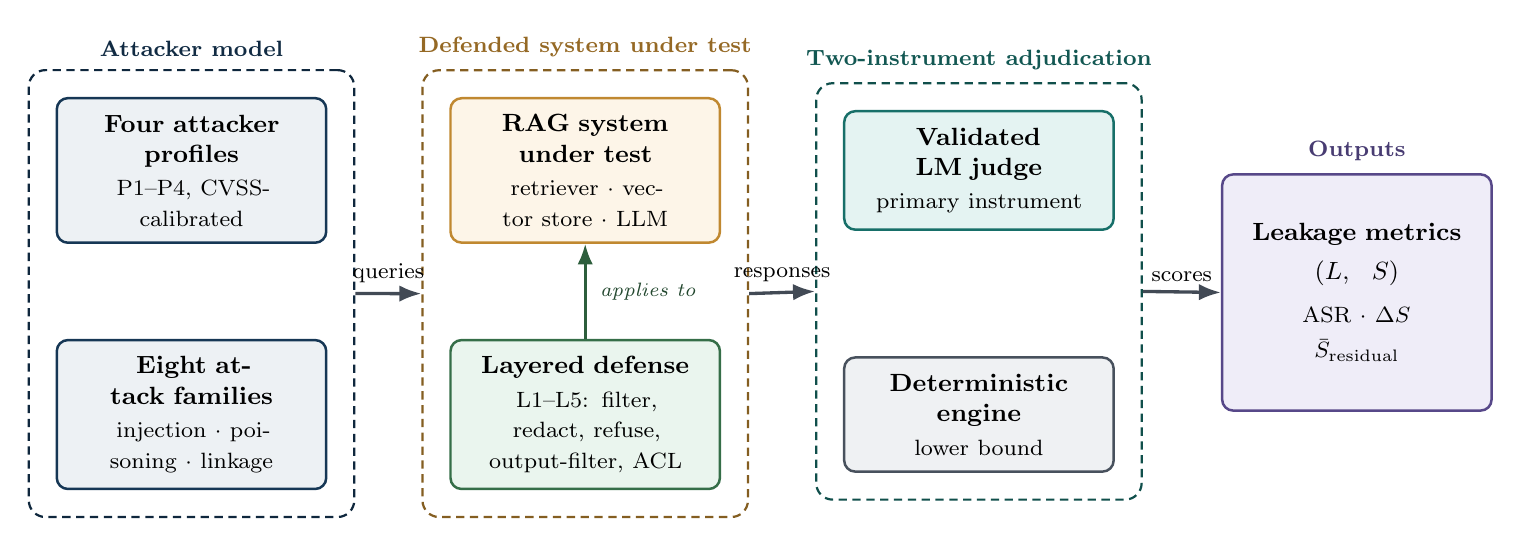
\begin{tikzpicture}[font=\small, >={Latex[length=2.8mm]},
  box/.style={rounded corners=4pt, draw, line width=0.9pt, align=center, inner sep=6pt,
    text width=30mm, minimum height=14mm},
  grp/.style={rounded corners=6pt, line width=0.8pt, dash pattern=on 3pt off 2pt, inner sep=3.4mm},
  glab/.style={font=\footnotesize\bfseries},
  ar/.style={-{Latex[length=2.8mm]}, line width=1.2pt, draw=figslate!55!black}]
% Stage A: attacker model
\node[box, fill=figblue!8, draw=figblue!70!black] (prof) at (0,1.55) {\textbf{Four attacker profiles}\\[1pt]\footnotesize P1--P4, CVSS-calibrated};
\node[box, fill=figblue!8, draw=figblue!70!black] (fam) at (0,-1.55) {\textbf{Eight attack families}\\[1pt]\footnotesize injection $\cdot$ poisoning $\cdot$ linkage};
\node[grp, draw=figblue!50!black, fit=(prof)(fam)] (attbox) {};
% Stage B: defended system under test
\node[box, fill=figamber!12, draw=figamber!80!black] (sut) at (5.0,1.55) {\textbf{RAG system under test}\\[1pt]\footnotesize retriever $\cdot$ vector store $\cdot$ LLM};
\node[box, fill=figgreen!12, draw=figgreen!65!black] (def) at (5.0,-1.55) {\textbf{Layered defense}\\[1pt]\footnotesize L1--L5: filter, redact, refuse, output-filter, ACL};
\node[grp, draw=figamber!55!black, fit=(sut)(def)] (sutbox) {};
% Stage C: two-instrument adjudication
\node[box, fill=figteal!12, draw=figteal!70!black] (judge) at (10.0,1.55) {\textbf{Validated LM judge}\\[1pt]\footnotesize primary instrument};
\node[box, fill=figslate!12, draw=figslate!60!black] (eng) at (10.0,-1.55) {\textbf{Deterministic engine}\\[1pt]\footnotesize lower bound};
\node[grp, draw=figteal!50!black, fit=(judge)(eng)] (adjbox) {};
% Stage D: leakage metrics
\node[box, fill=figviolet!12, draw=figviolet!70!black, text width=30mm, minimum height=30mm] (met) at (14.8,0) {\textbf{Leakage metrics}\\[3pt]$(L,\;S)$\\[6pt]\footnotesize ASR $\cdot$ $\Delta S$\\[2pt]$\bar S_{\text{residual}}$};
% main flow arrows, aligned on a single baseline between the stages
\draw[ar] (attbox.east) -- node[above, font=\footnotesize]{queries}   (sutbox.west);
\draw[ar] (sutbox.east) -- node[above, font=\footnotesize]{responses} (adjbox.west);
\draw[ar] (adjbox.east) -- node[above, font=\footnotesize]{scores}    (met.west);
% internal arrow: the layered defense is applied to the system under test
\draw[-{Latex[length=2.6mm]}, line width=0.95pt, draw=figgreen!55!black]
  (def.north) -- node[right=1.5pt, font=\scriptsize\itshape, text=figgreen!42!black]{applies to} (sut.south);
% stage captions above each group
\node[glab, text=figblue!55!black,   anchor=south, yshift=1pt] at (attbox.north) {Attacker model};
\node[glab, text=figamber!62!black,  anchor=south, yshift=1pt] at (sutbox.north) {Defended system under test};
\node[glab, text=figteal!55!black,   anchor=south, yshift=1pt] at (adjbox.north) {Two-instrument adjudication};
\node[glab, text=figviolet!58!black, anchor=south, yshift=1pt] at (met.north)    {Outputs};
\end{tikzpicture}}
\caption[The unified measurement framework]{The unified measurement framework. Four CVSS-calibrated
attacker profiles and eight attack families drive queries at the RAG system under test; a layered
defense (L1--L5) is ablated configuration by configuration; each response is adjudicated by a
validated language-model judge (primary) with a deterministic engine reported as a lower bound; and
both feed the profile-dependent leakage metrics $L$ and $S$.}
\label{fig:m-framework}
\end{figure}

\subsection{The two leakage metrics, formally}
\label{sec:intro-metrics}

Privacy leakage is given a precise foundation by two complementary, LINDDUN-aligned metrics. The
binary function $L$ answers \emph{whether} an unauthorized disclosure occurred; the continuous score
$S$ answers \emph{how severe} it was. Both are profile-dependent: the same response can be a leak for
one profile and authorized for another, because each profile carries its own authorization threshold.
The definitions below are the design contract; their empirical application is the subject of the
companion report.

\begin{defbox}[Definition 1: Binary privacy-leakage function $L(q,r,D,u)$]
For a query $q$, a system response $r$, the indexed document set $D$, and a user profile $u$ with
maximum authorized disclosure level $\textit{authorized\_level}(u)$,
\[
L(q,r,D,u)=
\begin{cases}
1 & \text{if } \exists\, x \in \textit{info}(r,D)\ \text{such that}\ \textit{severity}(x) > \textit{authorized\_level}(u),\\[2pt]
0 & \text{otherwise,}
\end{cases}
\]
where $\textit{info}(r,D)$ is the set of information items in $r$ that originate from $D$, and
$\textit{severity}(x)\in\{2,3,4,5\}$ is the item's severity weight from the leakage taxonomy. The
attack success rate over a batch of $N$ scenarios is $\mathrm{ASR}=\tfrac{1}{N}\sum_{i=1}^{N}L(q_i,r_i,D,u)$.
\end{defbox}

\begin{defbox}[Definition 2: Continuous severity score $S(q,r,D,u)$]
Let $E(r,D,u)=\bigl\{\, e \mid e\in\textit{entities}(r,D),\ \textit{severity}(e)>\textit{authorized\_level}(u)\,\bigr\}$
be the set of unauthorized PII entities disclosed in $r$. Then
\[
S(q,r,D,u)=\sum_{e\,\in\, E(r,D,u)} s(e)\cdot w(e),
\]
where $s(e)\in\{2,3,4,5\}$ is the entity's intrinsic severity and $w(e)\in[0,1]$ is a
detection-confidence weight (Regex $1.00$, NER $0.90$, keyword+context $0.75$, model-judge $0.60$)
that scales down probabilistically detected entities. Two derived quantities carry the empirical
argument: the \textbf{defense effectiveness} $\Delta S = S_{\text{baseline}}-S_{\text{defended}}$, and
the \textbf{residual risk} $\bar{S}_{\text{residual}}=\tfrac{1}{N}\sum_{i=1}^{N} S(q_i,r_i,D,u)$ with
the full defense stack active. By construction, $L=1 \Leftrightarrow S>0$.
\end{defbox}

\subsection{The four attacker profiles}
\label{sec:intro-profiles}

The threat surface is fixed in advance as four attacker profiles, each calibrated against a Common
Vulnerability Scoring System (CVSS) v3.1 base score and assigned an authorization threshold:
the severity level above which a disclosure counts as leakage for that profile (\Cref{tab:m-profiles}).
The profiles are never inferred from the query: each experimental batch is run under an explicitly
chosen profile, so the framework measures what the system \emph{would} disclose to each kind of threat
actor rather than building a user-classification system.

\begin{table}[H]
\centering
\caption{The four CVSS-calibrated attacker profiles that fix the threat surface. The authorization
threshold sets the severity level above which a disclosure counts as leakage for that profile; the
profiles, scores, and thresholds are developed in full in the companion report's threat model.}
\label{tab:m-profiles}
\small
\begin{tabularx}{\textwidth}{@{}llcL@{}}
\toprule
\textbf{Profile} & \textbf{CVSS v3.1} & \textbf{Auth.} & \textbf{What counts as leakage; primary attack vector} \\
\midrule
P1: Internal Employee     & 6.5 (medium)   & 2 & Severity $\geq 3$ from the corpus; social engineering via natural-language queries \\
P2: External Adversary    & 8.2 (high)     & 0 & \emph{Any} corpus disclosure; prompt injection, jailbreaking, obfuscation \\
P3: Privileged Admin      & 9.1 (critical) & 3 & Severity $\geq 4$ via chat; corpus poisoning, configuration exfiltration \\
P4: Third-Party Provider  & 7.7 (high)     & 3 & Aggregate / cross-tenant severity $\geq 4$; offline, bounded by an API contract \\
\bottomrule
\end{tabularx}
\end{table}

\subsection{The evaluation corpus}
\label{sec:intro-corpus}

The framework is exercised against a synthetic ground-truth corpus rather than real organizational
data, so that every reported figure is reproducible and no real person is exposed. The corpus
comprises \textbf{155 documents} in four classes (100 employee records, 30 medical reports, 20
internal memoranda, and 5 system-configuration files) generated deterministically with Python's
Faker library under a fixed seed (\texttt{random.seed(42)}, \texttt{Faker.seed(42)}), so the same
corpus is reproduced on every run and on any machine. Every document is then annotated at the entity
level, yielding \textbf{2{,}190 PII entities} (about 14 per document) drawn from a 36-type taxonomy
that spans direct identifiers (names, dates of birth, IBANs, national IDs), special-category data
(GDPR Article~9 medical conditions), and quasi-identifiers whose risk is combinatorial. Each entity
records its severity weight $s(e)\in\{2,3,4,5\}$ and the detection method that found it, which
together make $L$ and $S$ computable against an authoritative reference standard.

\textbf{A deliberate limitation.}\quad Faker produces records that are \emph{plausible} rather than
\emph{realistic}: attributes are sampled independently, so the corpus omits the statistical
correlations of real data (salaries clustering at mid-band values, medical conditions correlating with
age and occupation) and uses English-pattern names rather than Algerian Arabic naming conventions. The
only correlations present are those written in by design (medical reports linked to employee IDs,
memoranda referencing specific employees). This is precisely why the framework's findings are read as
relative and methodological, and the absolute percentages as a demonstration on a controlled corpus
rather than predictions for any real deployment.

\textbf{Reproducibility.}\quad Because the corpus, its annotations, and the evaluation engine are all
deterministic, every quantity in this line of work traces to a fixed artifact: the seed-42 corpus, the
2{,}190-entity annotation set, and the profile-dependent $(L,S)$ engine. The companion report records
the per-scenario logs and the judge cache from which its percentages are computed, so that any figure
can be re-derived rather than taken on trust.

\textbf{Data availability.}\quad Because the data is wholly synthetic, the corpus generator, its
entity-level annotations, and the profile-dependent evaluation engine carry no disclosure risk and
are available from the author on request; the full pipeline regenerates the identical 155-document
corpus from the fixed seed, so no real or third-party data is required to reproduce any result.

\section{Findings, honestly previewed}
\label{sec:intro-findings}

The companion final-year report's headline result is a genuine but partial reduction. Read through
the validated judge, the
primary instrument, the full defense stack reduces leakage from $28.8\%$ to $17.3\%$, a reduction
of roughly forty percent, \textbf{not an elimination}. (The deterministic engine, by contrast,
reports near-zero, which is exactly the single-instrument error described above.) The residual is
not uniform. Re-identification by \emph{linkage} is its dominant unreduced component: redaction
defeats direct extraction but cannot remove a person assembled from scattered attributes.
The instrument that delivers the headline is
itself bounded, and its reliability was established by protocol rather than assumed. On a 46-record
calibration sample labeled by two human annotators (who agreed with each other at Cohen's
$\kappa = 0.692$), the judge agreed with the primary human annotator at $\kappa = 0.827$ on
undefended output, at least as closely as the second annotator did, comfortably clearing the
$\kappa \geq 0.60$ validation gate. On the defended distribution the numbers are built from, that
agreement falls to $\kappa = 0.306$, a single-annotator exposure the companion report records and its
future work names. The $17.3\%$ figure is therefore reported with an honest uncertainty interval, and
the tempting claim that the true rate is \emph{lower} is refused. (The full validation protocol, covering the
calibration sample, annotator agreement, and the deterministic engine's $\kappa = 0.164$ that exposes
its false-positive tendency, is reported in the companion final-year report.) The whole is best read as
\textbf{a demonstration of a measurement methodology on a controlled, synthetic corpus, not a
certification that any deployable system is safe}: the relative findings (which layer matters,
which adversary is hardest, how the residual is composed) are what transfer; the absolute
percentages are not predictions.

\section{Thesis structure}
\label{sec:intro-structure}

This report is organized as follows. The present chapter has set out the context, the problem,
the research gap, the research questions, and the contribution, and has \emph{designed} the
measurement framework: the formal $(L,S)$ metrics, the four attacker profiles, and the evaluation
corpus. Chapter~\ref{ch:sota} surveys forty-nine primary sources across the five pillars.
Chapter~\ref{ch:comparative} draws them into a comparative analysis and identifies the research gap
that motivates the framework. Chapter~\ref{ch:conclusion} concludes by drawing the survey and the
framework together, and states the limitations of this report explicitly. The full threat model, the
adversarial campaign, and the complete experimental evaluation are reported in the companion
final-year (PFE) report; \Cref{fig:m-scope} summarizes the division of labor between the two
documents.

\begin{figure}[H]
\centering
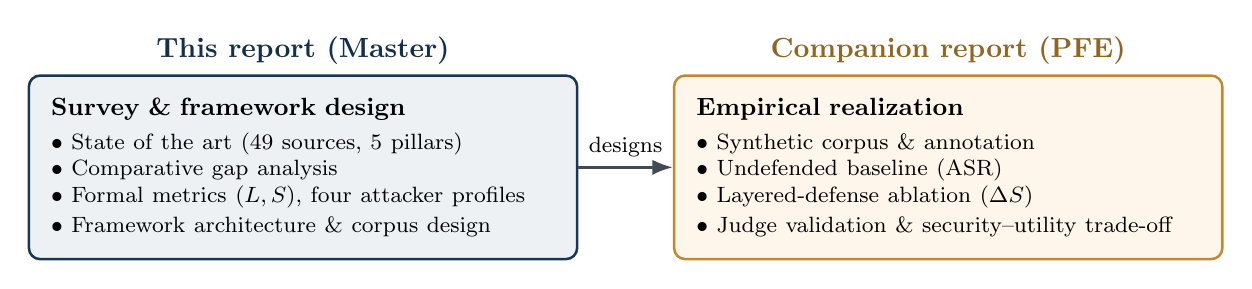
\begin{tikzpicture}[font=\small,
  box/.style={rounded corners=4pt, draw, line width=0.9pt, align=left, inner sep=8pt, text width=64mm}]
\node[box, fill=figblue!8, draw=figblue!70!black,
  label={[font=\bfseries\color{figblue!60!black}]above:This report (Master)}] (m)
  {\textbf{Survey \& framework design}\\[3pt]
   \footnotesize $\bullet$~State of the art (49 sources, 5 pillars)\\
   $\bullet$~Comparative gap analysis\\
   $\bullet$~Formal metrics $(L,S)$, four attacker profiles\\
   $\bullet$~Framework architecture \& corpus design};
\node[box, fill=figamber!10, draw=figamber!80!black, right=12mm of m,
  label={[font=\bfseries\color{figamber!60!black}]above:Companion report (PFE)}] (p)
  {\textbf{Empirical realization}\\[3pt]
   \footnotesize $\bullet$~Synthetic corpus \& annotation\\
   $\bullet$~Undefended baseline (ASR)\\
   $\bullet$~Layered-defense ablation ($\Delta S$)\\
   $\bullet$~Judge validation \& security--utility trade-off};
\draw[-{Latex[length=2.6mm]}, line width=1pt, draw=figslate!55!black]
  (m.east) -- node[above, font=\footnotesize]{designs} (p.west);
\end{tikzpicture}
\caption[Division of labor between the two reports]{Division of labor between this Master report
and the companion final-year (PFE) report. This report surveys the field, isolates the research gap,
and \emph{designs} the measurement framework; the companion report carries out its empirical
realization. The empirical percentages quoted here are companion findings, included only as context.}
\label{fig:m-scope}
\end{figure}


%%%%%%%%%%%%%%%%%%%%%%%%%%%%%%%%%%%%%%%%%%%%%%%%%%%%%%%%%%%%%%%%%%%%%%%%%%%%%%
% ===== State of the Art =====
%%%%%%%%%%%%%%%%%%%%%%%%%%%%%%%%%%%%%%%%%%%%%%%%%%%%%%%%%%%%%%%%%%%%%%%%%%%%%%
\chapter{State of the Art}
\label{ch:sota}

\section*{Introduction}
\phantomsection
\addcontentsline{toc}{section}{Introduction}
\label{sec:soa-intro}

When large language models (LLMs) are coupled with external knowledge retrieval, what we now call Retrieval-Augmented Generation (RAG), a new class of privacy and security concerns emerges that neither the LLM safety community nor the information retrieval community has fully tackled on its own. On one side, the evidence that language models memorize verbatim fragments of training data, including personally identifiable information (PII), is by now incontrovertible. On the other, prompt injection has been shown to steer LLM behavior through cleverly crafted adversarial inputs. The substantive research problem sits in the collision of these two phenomena inside a RAG pipeline, where an LLM generates answers based on dynamically retrieved documents that may contain sensitive data. The resulting attack surface is larger than the union of the individual surfaces, because the retriever itself becomes an attacker-controllable channel. \Cref{fig:m-attack-surface} maps that surface onto the enterprise-RAG pipeline and marks where each attacker profile enters it.

\begin{figure}[H]
\centering
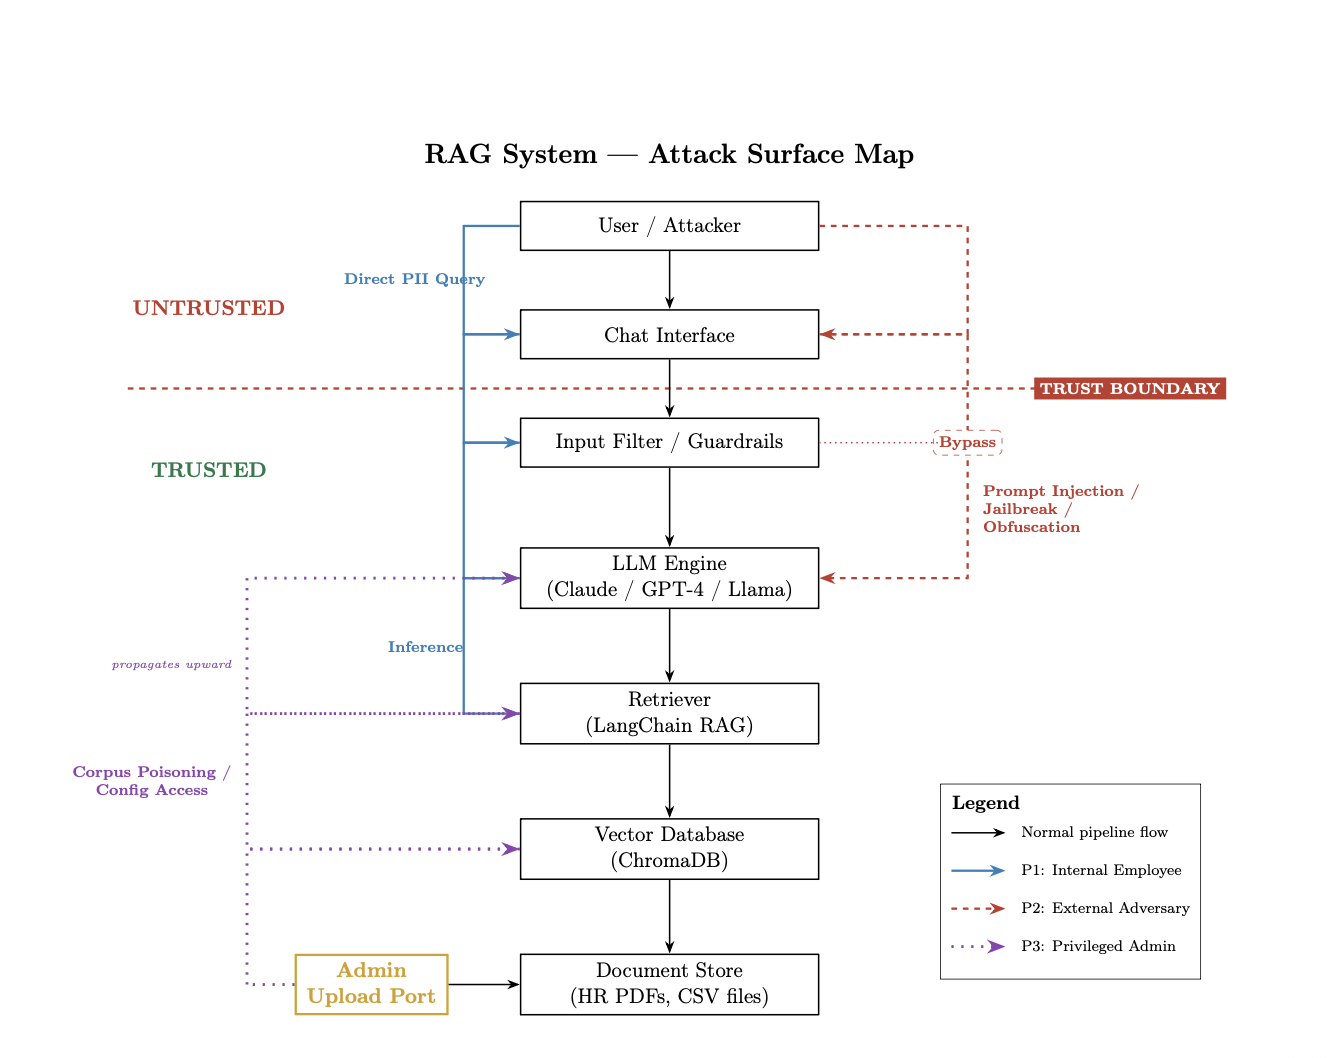
\includegraphics[width=0.9\textwidth]{fig_attack_surface_map.png}
\caption[The RAG attack surface and its privacy-leakage points]{The enterprise-RAG pipeline and where
privacy leakage enters it. A query flows from the user through the input guardrails, the LLM engine,
the retriever, the vector database, and the document store; the trust boundary separates untrusted
callers from the trusted corpus. Each of the three live attacker profiles exercises a different entry point: an internal
employee (P1) issues direct PII queries, an external adversary (P2) injects instructions across the
boundary, and a privileged admin (P3) poisons the corpus or exfiltrates configuration upward through
the store.}
\label{fig:m-attack-surface}
\end{figure}

This chapter is a structured, critical walk through the literature sitting at that intersection. Rather than a chronological reading of papers, the review is organized around five thematic pillars that together map out the research territory surrounding this thesis:

\begin{enumerate}[leftmargin=2em, itemsep=3pt]
  \item \textbf{RAG-Specific Vulnerabilities} (\Cref{sec:rag-vuln}): how the retrieval--generation pipeline opens up attack surfaces (indirect prompt injection, corpus poisoning, retriever-layer backdoors) that simply do not exist in standalone LLM deployments.
  \item \textbf{PII Memorization and Leakage in LLMs} (\Cref{sec:pii-leakage}): the evidence that language models memorize training data, the scaling laws that govern this phenomenon, and the growing distinction between memorization-based and reasoning-based privacy violations.
  \item \textbf{Prompt Injection Taxonomies and Attack Families} (\Cref{sec:pi-taxonomy}): the classification schemes proposed for the fast-growing space of adversarial prompt techniques, from the OWASP industry standard to academic systematizations.
  \item \textbf{Defense Mechanisms and Guardrail Architectures} (\Cref{sec:defenses}): protective measures ranging from static input filters to programmable guardrail toolkits and multi-agent safety frameworks.
  \item \textbf{LLM-as-Judge and Multi-Agent Evaluation} (\Cref{sec:llm-judge}): using language models to evaluate other language models, and the shift toward multi-agent debate and arbitration.
\end{enumerate}

\Cref{fig:m-pillars} shows the five pillars and the research gap that opens at their intersection.

\begin{figure}[H]
\centering
\resizebox{\textwidth}{!}{%
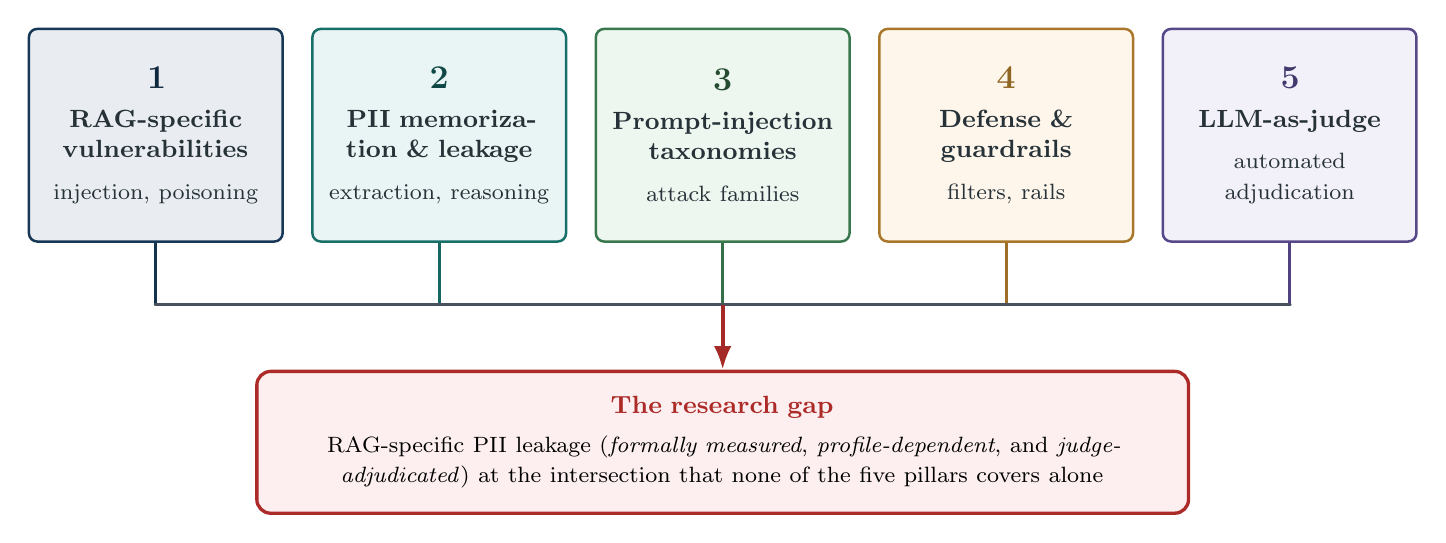
\begin{tikzpicture}[font=\small, >={Latex[length=2.6mm]},
  pil/.style 2 args={rounded corners=3pt, draw=#1!70!black, fill=#1!10, line width=0.9pt,
    align=center, inner sep=6pt, text width=28mm, minimum height=27mm, text=darkcharcoal}]
\node[pil={figblue}{}]   (p1) at (0,0)    {{\bfseries\large\textcolor{figblue!50!black}{1}}\\[3pt]\textbf{RAG-specific vulnerabilities}\\[4pt]\footnotesize injection, poisoning};
\node[pil={figteal}{}]   (p2) at (3.6,0)  {{\bfseries\large\textcolor{figteal!45!black}{2}}\\[3pt]\textbf{PII memorization \& leakage}\\[4pt]\footnotesize extraction, reasoning};
\node[pil={figgreen}{}]  (p3) at (7.2,0)  {{\bfseries\large\textcolor{figgreen!45!black}{3}}\\[3pt]\textbf{Prompt-injection taxonomies}\\[4pt]\footnotesize attack families};
\node[pil={figamber}{}]  (p4) at (10.8,0) {{\bfseries\large\textcolor{figamber!60!black}{4}}\\[3pt]\textbf{Defense \& guardrails}\\[4pt]\footnotesize filters, rails};
\node[pil={figviolet}{}] (p5) at (14.4,0) {{\bfseries\large\textcolor{figviolet!55!black}{5}}\\[3pt]\textbf{LLM-as-judge}\\[4pt]\footnotesize automated adjudication};
% the research gap, at the intersection of all five pillars
\node[rounded corners=5pt, draw=accentcolor!75!black, fill=accentcolor!8, line width=1.2pt,
  align=center, inner sep=9pt, text width=112mm] (gap) at (7.2,-3.9)
  {\textbf{\textcolor{accentcolor!75!black}{The research gap}}\\[3pt]\footnotesize RAG-specific PII
   leakage (\emph{formally measured}, \emph{profile-dependent}, and \emph{judge-adjudicated})
   at the intersection that none of the five pillars covers alone};
% aligned, colour-matched vertical drops from each pillar to the collector bus
\foreach \p/\x/\col in {p1/0/figblue, p2/3.6/figteal, p3/7.2/figgreen, p4/10.8/figamber, p5/14.4/figviolet}
  \draw[line width=1pt, draw=\col!65!black] (\p.south) -- (\x,-2.15);
% horizontal collector bus joining the five drops
\draw[line width=1.4pt, draw=figslate!60!black, line cap=round] (0,-2.15) -- (14.4,-2.15);
% single merge arrow from the bus centre into the gap box
\draw[-{Latex[length=3mm]}, line width=1.5pt, draw=accentcolor!72!black] (7.2,-2.15) -- (gap.north);
\end{tikzpicture}}
\caption[The five literature pillars and the gap at their intersection]{The five thematic pillars
surveyed in this chapter and the research gap that emerges at their intersection: the point where
RAG-specific attacks meet PII-specific privacy metrics, a formal threat taxonomy, layered defenses,
and automated leak adjudication. Each pillar is mature within its own boundary; none addresses their
convergence.}
\label{fig:m-pillars}
\end{figure}

Each pillar ends with an explicit list of the methodological gaps the current literature leaves open. \Cref{sec:synthesis} then pulls these together into a unified research positioning statement, including a single sentence that captures the original contribution of this thesis relative to the forty-nine surveyed works.

\begin{notebox}
\textbf{A note on 2026 references.} This thesis surveys a fast-moving field. Some 2026 citations are arXiv preprints that have not yet completed peer review, while others are peer-reviewed journal publications. The principal 2026 works are footnoted at first mention with their verified publication status (peer-reviewed entries cite their DOI; preprints cite their arXiv identifier), and all 2026 entries are listed with their status in the References. Preprints are admissible evidence for a literature review of an emerging field, but their claims are treated as provisional.
\end{notebox}


% ══════════════════════════════════════════════════════════
%  2 — RAG VULNERABILITIES
% ══════════════════════════════════════════════════════════

\newpage
\section{RAG-Specific Vulnerabilities}
\label{sec:rag-vuln}

\subsection{The Emergence of Indirect Prompt Injection}

The work that really kicked things off was by Greshake et al.\ (2023), who introduced and formalized \emph{Indirect Prompt Injection} (IPI) as a new class of attack aimed specifically at systems that pull in external content and pass it to an LLM. The key difference from direct prompt injection is that the adversary does not tamper with the user's input. Instead, they plant adversarial instructions inside documents that the retriever picks up later. Using qualitative demonstrations on Bing Chat, Greshake et al.\ showed that a RAG system could be tricked into following arbitrary instructions hidden in third-party web pages. The threat model for any LLM-integrated application that consumes external data was changed from that point on.

\begin{critbox}
\textit{Reading this paper carefully}, one notices that its contribution is conceptual rather than empirical. The paper is a threat-model manifesto supported by proof-of-concept demonstrations, not a controlled benchmark. Its lasting value is the vocabulary it gave the field (the IPI paradigm) rather than measurable attack-success figures, and any subsequent work that cites it as empirical evidence overstates what was actually demonstrated.
\end{critbox}

Before Greshake et al., Perez and Ribeiro (2022) had already laid some conceptual groundwork by formalizing \emph{Goal Hijacking} and \emph{Prompt Leaking} as distinct attack objectives in the direct-injection setting, and by introducing the PROMPTINJECT testing framework. Their approach, assembling prompts in a modular way and systematically swapping injection payloads across 35 application scenarios, gave us the first quantitative baselines for how often direct prompt injection actually succeeds.

\begin{critbox}
\textit{PROMPTINJECT matters as the methodological ancestor of measurable injection evaluation}, and its modular payload-swapping pattern is the one we reuse in Phase 2. The scope, however, is strictly the user-input channel. The retrieval context is out of frame, which means PROMPTINJECT cannot be transposed to indirect attacks without substantive extension: the injection no longer originates from a user we can model but from a document we cannot necessarily trust.
\end{critbox}

\subsection{From Qualitative Demonstrations to Quantitative Benchmarking}

Systematic benchmarking, as opposed to scattered demonstrations, is largely the contribution of Yi et al.\ (2025), who built the \textbf{BIPIA} benchmark. This was the first large-scale dataset designed specifically to test the robustness of LLMs against indirect prompt injection. Their core insight was pinpointing \emph{instruction vs.\ data confusion} as the root cause of IPI. The LLM cannot distinguish between instructions issued by the system and content pulled from retrieved documents. Quantitative evaluation across GPT, Llama, and Vicuna families showed every model tested to be significantly vulnerable, with attack-success rates varying by model architecture and document type.

\begin{critbox}
\textit{Genuine methodological advance here}: BIPIA moves the field from anecdote to reproducible measurement. The benchmark is, however, task-centric rather than privacy-centric. Attack success is defined at the level of ``did the injected instruction execute?'', which is not the same question as ``did a sensitive entity get disclosed?''. Applied directly to RAG privacy, BIPIA is a useful precedent for reproducibility discipline, but its task-completion metric has to be swapped out for a PII-specific severity score $S$ to match the thesis's privacy focus.
\end{critbox}

Liu et al.\ (2025) then pushed the attacker methodology further with \textbf{HOUYI}, an iterative three-component attack system (Framework Component, Separator, Disruptor) built for black-box exploitation of commercial applications. Tested across 36 real-world services, HOUYI broke production systems even when they had multiple defense layers.

\begin{critbox}
\textit{HOUYI is the technical blueprint for the Attacker Agent}, with one caveat that matters a lot in practice. HOUYI optimizes for task-hijack success. The thesis's Attacker Agent has to optimize for PII-specific disclosure, a weaker and subtler signal than generic task completion. Directly replicating HOUYI would maximize the wrong objective, so the reward function has to be redesigned from scratch.
\end{critbox}

\subsection{Corpus Poisoning and Retriever-Layer Attacks}

A parallel category of RAG vulnerability targets not the prompt but the data-ingestion layer. Xue et al.\ (2024) found that an adversary with write access to the knowledge base can craft specially optimized passages (using Corpus Optimization Procedures, COP/MCOP) that reliably land in top retrieval positions, letting the attacker control the context fed to the LLM. Their work also introduced \emph{Alignment as an Attack} (AaaA), showing that the very mechanism meant to make LLMs helpful can be turned against them. Clop and Teglia (2024) went further by targeting the retriever itself, demonstrating that fine-tuning backdoors can be planted directly in the embedding model. Their controlled comparison on Llama-3 and Mistral showed the retriever-layer attacks to be stealthier and harder to detect than prompt-level alternatives.

\begin{critbox}
\textit{What these two papers share is a blind spot}: both stop at generic corpus manipulation, and neither asks whether the poisoning payload can be engineered to extract a specific category of PII on demand. In enterprise RAG the practical threat is not output manipulation in the generic sense. It is an attacker using corpus poisoning to systematically drain HR, medical, or financial records. Our Privileged Admin profile (P3) targets exactly this shift from output manipulation to targeted PII exfiltration, which the existing literature does not operationalize.
\end{critbox}

\subsection{Formal Threat Modeling and Adversarial Foundations}

Perhaps the most theoretically ambitious contribution to RAG security is Arzanipour et al.\ (2025), who present the first formal threat model with rigorous mathematical definitions for RAG-specific privacy threats, including Membership Inference and corpus poisoning. They develop a two-dimensional adversary taxonomy (Model Access $\times$ Adversarial Knowledge) along with document-level differential-privacy definitions.

\begin{critbox}
\textit{The Arzanipour paper reads as the theoretical counterpart to our empirical framework}: they provide the definitions, we provide the ground truth. The authors themselves are up-front about the limitation, which is that the paper offers no large-scale empirical test of its formalisms. This asymmetry between formal theory and empirical validation is exactly the gap this thesis positions itself to close for a targeted subset of the space, namely PII leakage under four attacker profiles.
\end{critbox}

At the model level, Wei et al.\ (2023) gave us the theoretical basis for understanding \emph{why} safety-aligned LLMs remain vulnerable even after training-time interventions. They pinpointed two fundamental failure modes of LLM safety training, \emph{Competing Objectives} and \emph{Mismatched Generalization}, and showed through hypothesis-driven jailbreak experiments (Prefix Injection, Base64 encoding) on GPT-4 and Claude v1.3 that these predictions hold up empirically. Their focus is model-level safety rather than RAG-specific threats, but the failure-mode taxonomy directly shapes the Attacker Agent's strategy selection in this thesis: each attack family in our design exploits one or both of the failure modes they described.

\subsection{Contemporary Synthesis and Pillar Assessment}

The most recent comprehensive overview of the RAG vulnerability landscape is Gulyamov et al.\ (2026)\footnote{Peer-reviewed journal article. Published in \emph{Information} 17(1), art.~54 (MDPI), received 25 Oct 2025, accepted 31 Dec 2025, published online 7 Jan 2026, as part of the special issue ``Emerging Trends in AI-Driven Cyber Security and Digital Forensics.'' DOI \href{https://doi.org/10.3390/info17010054}{10.3390/info17010054}. A preceding preprint exists on Preprints.org, but the journal version is the version of record.}, who compile a taxonomy of direct and indirect attacks alongside the \textbf{PALADIN} five-layer defense framework. Their systematic review covers 45 primary sources and industry CVEs from 2023--2025, and documents notable real-world incidents including GitHub Copilot's CVE-2025-53773 (CVSS 9.6) and the CamoLeak exploit.

\begin{critbox}
\textit{Being a secondary study, PALADIN contributes no original empirical data.} For our purposes that makes it a landscape counterpart rather than a benchmark. PALADIN maps what practitioners think defense-in-depth should look like. The thesis measures what defense-in-depth actually achieves under controlled PII-specific ground truth. The two frameworks are therefore methodologically orthogonal. PALADIN answers ``what layers should exist?'' while this thesis answers ``what does the security-utility trade-off actually look like when you deploy them?'' One additional caveat is worth recording: the paper's author affiliations are predominantly in law departments rather than computer-security labs, which is atypical for a technical defense framework and is one reason we treat it as a landscape reference rather than a primary empirical source.
\end{critbox}

\begin{gapbox}[Residual Gaps, RAG Vulnerabilities]
Despite all the progress covered above, four methodological gaps remain in this pillar:
\begin{enumerate}[leftmargin=1.5em, itemsep=3pt]
  \item No study so far has used a formal privacy framework (such as LINDDUN) to categorize RAG-specific leakage events by threat type and severity.
  \item Quantitative benchmarking of PII leakage rates, as a distinct concern from general task hijacking or information steering, is still missing.
  \item Nobody has yet implemented an automated multi-agent evaluation setup to systematically measure how different attack families interact with different defense configurations.
  \item The formal threat models proposed by Arzanipour et al.\ have not been put to the test against a controlled ground-truth corpus.
\end{enumerate}
\end{gapbox}

% ── TRANSITION FROM PILLAR 1 TO PILLAR 2 ──
\begin{transitionbox}[Transition from Pillar 1 to Pillar 2]
Pillar 1 has established the \emph{channel}: how the retrieval--generation pipeline opens an
attacker-controllable path into the model's context. On its own, though, a channel is empty. What
makes it dangerous is the \emph{payload} it can carry: the sensitive content the model actually
holds and can be made to emit. Pillar 2 supplies exactly that. It assembles the evidence that
language models memorize verbatim fragments of their training data, that this memorization scales
with model capacity and context length, and that, more recently, instruction-following and reasoning
can reconstruct private data even when verbatim memorization is low. The two pillars therefore
compose: Pillar 1 is the delivery mechanism, Pillar 2 is the substance delivered, and the RAG-specific
threat this thesis measures is precisely their product. The review now turns from how leakage is
\emph{triggered} to what there is to leak.
\end{transitionbox}


% ══════════════════════════════════════════════════════════
%  3 — PII LEAKAGE IN LLMs
% ══════════════════════════════════════════════════════════

\newpage
\section{PII Memorization and Leakage in Large Language Models}
\label{sec:pii-leakage}

\subsection{Foundational Evidence of Training Data Memorization}

The landmark study by Carlini et al.\ (2021) was the one that proved LLMs memorize word-for-word fragments of their training data, including PII such as names, phone numbers, email addresses, and physical addresses. The authors generated over 200{,}000 samples from GPT-2, checked them against internet sources and known training corpora, and showed that memorization is not a rare fluke but a systematic property of how neural language models work. The likelihood-ratio method they used for ranking and spotting leaked sequences remains the canonical extraction methodology.

In a follow-up, Carlini et al.\ (2023) discovered that memorization scales log-linearly with three factors: model capacity, how often data gets repeated, and context length.

\begin{critbox}
\textit{Both Carlini papers are foundational}, but they measure memorization of a static model in isolation. There is no retriever, no user query, no downstream task. For RAG the third scaling factor, context length, is the most worrying one, because a retriever routinely supplies the model with long, context-rich prefixes from the organizational knowledge base. Carlini et al.'s own findings therefore \emph{imply} that RAG should amplify PII extraction without \emph{demonstrating} it. Nakka et al.\ (\S\ref{subsec:rag-amplification}) later fill in the experimental gap, and the thesis operationalizes the effect under controlled ground truth.
\end{critbox}

\subsection{Beyond Verbatim Memorization: Reasoning-Based Leakage}

An important shift came from Sander et al.\ (2025), who showed that instruction-following capability, rather than raw verbatim memorization, is what drives most PII leakage in chat-based deployments. By fine-tuning LLMs on synthetic PII and comparing raw memorization (prefix completion) against chat-based extraction (question-answering), they found the chat modality pulls out considerably more PII. The model's reasoning and instruction-following abilities can therefore be weaponized to reconstruct private data even when verbatim memorization is low.

Mireshghallah and Li (2025) reinforced this through a longitudinal review of 1{,}322 AI/ML privacy papers published between 2016 and 2025. They documented a strong ``memorization bias'' in the community: most privacy studies focus on verbatim extraction, while \emph{Context Leakage} and \emph{Aggregation}, the exact mechanisms that matter most for RAG, have barely been studied.

\begin{critbox}
\textit{Sander et al.\ deliver what is likely the most consequential empirical result for this thesis}, because the finding directly undermines the assumption that ``don't memorize PII'' is a sufficient defense strategy. If reasoning alone suffices to reconstruct private data, then model-level privacy guarantees (differential privacy, unlearning) are insufficient, and pipeline-level defenses become essential. Mireshghallah \& Li's position paper names the gap but offers no empirical testbed, which is what the thesis's 2{,}190-entity ground-truth corpus is designed to fill.
\end{critbox}

\subsection{The RAG Amplification Effect}
\label{subsec:rag-amplification}

Nakka et al.\ (2024) provided direct experimental evidence that external context makes memorized-data extraction worse. Working with GPT-J-6B and the Enron email corpus, they showed that \emph{in-domain grounding}, which means feeding the model unrelated text from the same dataset, drastically boosts the extraction of memorized PII such as phone numbers and email addresses. The authors did not, however, examine whether a normal, benign RAG pipeline might unintentionally produce this grounding effect as a side-effect of ordinary retrieval.

\begin{critbox}
\textit{This is a sharp illustration of how ``offensive research'' scenarios fail to capture the dual-use risk of RAG.} The same retrieval mechanism that improves answer quality in the benign case acts as an unintentional extraction primer in the adversarial one. Our benign-retrieval baseline (zero prompt injection, no corpus poisoning) is specifically designed to quantify this effect, which is a dimension Nakka et al.\ do not cover.
\end{critbox}

\subsection{Inherited Risks and the Unlearning Paradox}

Zhang et al.\ (2025) showed that knowledge distillation, a widely used technique for producing smaller, faster models, carries over the memorization and membership-inference risks from the teacher model. Borkar (2023) uncovered a related and rather troubling problem: fine-tuning not only keeps pre-training leaks intact but can introduce new ones, and attempts to ``unlearn'' specific data can sometimes backfire, making previously safe information vulnerable. This is what the author calls an \emph{unlearning paradox}.

\begin{critbox}
\textit{Zhang et al.\ and Borkar together build a strong negative case}: post-hoc model-level fixes for privacy leakage are structurally unreliable. The observation matters because it is the strongest available argument for moving the locus of defense from the model weights to the RAG pipeline (guardrails, sanitization, output filtering, judges), which is precisely the architectural stance of this thesis.
\end{critbox}

\subsection{Automated Red-Teaming and Agent-Based Extraction}

The most recent development in this area is the shift from manual extraction to automated, agent-driven red-teaming. Nie et al.\ (2025) built \textbf{LeakAgent}, a reinforcement-learning-based attacker that figures out extraction strategies on its own through Proximal Policy Optimization (PPO). Trained as a Llama-3-8B agent going after GPT-3.5, LeakAgent showed that automated agents can stumble upon novel attack strategies that human red-teamers miss entirely. Wang et al.\ (2025a) extended this kind of work to interaction memory, identifying \emph{Interaction Memory} as a privacy risk distinct from training memory and introducing the MEXTRA attack. Li et al.\ (2024a) built \textbf{LLM-PBE}, a unified toolkit benchmarking data extraction, membership inference, and PII leakage across more than ten open-source model families.

\begin{critbox}
\textit{LeakAgent proves the feasibility of an autonomous attacker}, and its methodology is the direct precedent for our Attacker Agent. The paper operates, however, in an open environment with no defender and no judge, and a complete evaluation needs all three. LLM-PBE treats the model as static and does not account for the dynamic retrieval interactions of a RAG pipeline. The thesis's Attacker-Defender-Arbitrator loop is designed to combine LeakAgent's autonomy with LLM-PBE's benchmark discipline inside a RAG architecture, a combination neither paper attempts.
\end{critbox}

\begin{gapbox}[Residual Gaps, PII Leakage]
\begin{enumerate}[leftmargin=1.5em, itemsep=3pt]
  \item Current studies look at memorization within model weights in isolation. None of them examines how context provided by a RAG retriever interacts with internal memorization to amplify or redirect leakage.
  \item No study has used a multi-agent ecosystem (Attacker + Defender + Arbitrator) to autonomously discover, defend against, and judge PII leaks in a RAG pipeline.
  \item The legal severity of leaks (GDPR Article classification, LINDDUN threat category) is not taken into account in any existing benchmark.
  \item The ``reasoning-based leakage'' that Sander et al.\ identified has not been tested within a RAG architecture where the retriever supplies the contextual grounding.
\end{enumerate}
\end{gapbox}

% ── TRANSITION FROM PILLAR 2 TO PILLAR 3 ──
\begin{transitionbox}[Transition from Pillar 2 to Pillar 3]
Pillars 2 and 3 can be confused because both describe scenarios in which sensitive information ends up in model output. The distinction this thesis uses throughout is the following. Pillar 2 is about \emph{what} can leak: it identifies the content that models retain (verbatim memorization, reasoning-reconstructable inferences, context-grounded recombinations) and documents the conditions under which that content becomes retrievable. In short, it is a theory of the leakage substrate. Pillar 3 is about \emph{how} an adversary causes leakage: it identifies the grammar of adversarial input (direct injection, indirect injection, obfuscation, jailbreaking, manipulation level) and classifies the techniques by which an attacker can exercise that substrate. It is a theory of the leakage trigger. Inside an attack pipeline, Pillar 3 techniques are the verbs and Pillar 2 phenomena are the objects. A prompt-injection payload (Pillar 3) is only dangerous insofar as it can mobilize a memorized or reasoning-reconstructable entity (Pillar 2) into the response. The thesis uses this distinction operationally: the Attacker Agent is parameterized over a Pillar 3 technique set, and success is measured against a Pillar 2 disclosure signal.
\end{transitionbox}


% ══════════════════════════════════════════════════════════
%  4 — PROMPT INJECTION TAXONOMY
% ══════════════════════════════════════════════════════════

\newpage
\section{Prompt Injection: Taxonomies and Attack Families}
\label{sec:pi-taxonomy}

\subsection{Industry-Standard Classification}

The \textbf{OWASP Top 10 for LLM Applications (2025)} set the main industry taxonomy, formally separating Direct Prompt Injection (LLM01) from Indirect Prompt Injection as the two principal attack categories. The classification was put together through a collaborative effort involving security practitioners worldwide, and it serves as the structural backbone for both academic research and industry mitigation work.

\begin{critbox}
\textit{OWASP is a static reference document}, with no empirical benchmarks, no automated testing methodology, no reproducibility clause. Its value is normative in the sense that it standardizes vocabulary for the community, but it measures nothing. For an experimental thesis that makes OWASP a mapping target rather than an evaluation yardstick, and that is exactly how we use it.
\end{critbox}

\subsection{Academic Systematizations}

Duarte et al.\ (2026)\footnote{Peer-reviewed journal article. Published in \emph{IEEE Access}, vol.~14, pp.~12875--12899 (2026). DOI \href{https://doi.org/10.1109/ACCESS.2026.3656849}{10.1109/ACCESS.2026.3656849}. \emph{IEEE Access} is an open-access peer-reviewed journal.} propose a taxonomy built on four manipulation levels (character, word, sentence, and semantic) crossed with adversarial intent, paying particular attention to how attacks escalate from simple string substitutions to complex semantic manipulations that exploit the model's reasoning. The paper also covers indirect injections via JSON/XML and tool-assisted or multimodal exploits.

Correia et al.\ (2026)\footnote{arXiv preprint, not peer-reviewed as of April 2026. arXiv:2601.22240 [cs.CR], submitted 29 Jan 2026. Available at \url{https://arxiv.org/abs/2601.22240}. No DOI has been minted. The manuscript uses an Elsevier-style template, but no evidence of submission, acceptance, or publication at a peer-reviewed venue was found.} assembled what appears to be the largest catalog of prompt-injection defenses currently available, analyzing 88 primary studies and sorting the interventions into training-time, deployment-time, and evaluation-time categories. They propose an expanded NIST taxonomy that stands as the most thorough defensive classification we have seen. One especially telling finding is that specialized interventions against indirect prompt injection, the kind that matters most for RAG systems, remain significantly underexplored relative to defenses against direct injection.

Wang et al.\ (2026)\footnote{arXiv preprint (Systematization of Knowledge), not peer-reviewed as of April 2026. arXiv:2602.10453 [cs.CR, cs.CL], submitted 11 Feb 2026. Available at \url{https://arxiv.org/abs/2602.10453}. The first author's own homepage labels the work as an arXiv preprint. The SoK format is typically submitted to top-tier security venues (IEEE S\&P, USENIX Security, CCS, NDSS), though no evidence of acceptance was located.} produced an extensive Systematization of Knowledge for LLM-agent prompt injection. They introduced the \textbf{AgentPI} benchmark and identified the \emph{Security-Utility-Latency trilemma}, a three-way trade-off that every practical defense deployment has to contend with. Their headline empirical finding is that no current defense simultaneously achieves high trustworthiness, high utility, and low latency, and that many apparently effective defenses work only by suppressing contextual inputs that real-world agents legitimately depend on.

\begin{critbox}
\textit{Read collectively}, Duarte et al., Correia et al., and Wang et al.\ form the most up-to-date picture of the attack and defense landscape, and between them they partition the space cleanly: Duarte on attack mechanics, Correia on defenses, Wang on agent-context evaluation. The three works share a limitation that is critical for our purposes, however. None of them speaks the language of privacy. Duarte et al.\ classify attacks by linguistic manipulation level. Correia et al.\ classify defenses by lifecycle stage. Wang et al.\ identify a performance trilemma. What is missing from all three is a mapping to privacy-specific outcomes: which attack family causes which category of PII to leak, under which formal threat model, evaluated against which regulatory baseline (GDPR article, LINDDUN category). That is the gap Pillar 1's LINDDUN-mapped taxonomy and Pillar 3's attack-to-leakage mapping together close. A further observation matters on the epistemic side: two of the three works remain preprints, so their claims carry less evidential weight than the peer-reviewed Duarte et al.\ paper, and the thesis treats them accordingly.
\end{critbox}

\subsection{Evolutionary Perspectives}

Mao et al.\ (2025) traced how the attack surface has evolved from text-only LLMs through multimodal models to autonomous-agent systems, introducing a permission-based jailbreak taxonomy that reflects the growing capabilities and risks of each architectural generation. Yi et al.\ (2024), in a survey distinct from the BIPIA work, proposed a complementary dual-axis taxonomy that organizes attacks by target-model transparency (Black-box vs.\ White-box) and defenses by intervention level (Prompt-level vs.\ Model-level). Schulhoff et al.\ (2023) contributed a classification based on source and goal, distinguishing attacks by where they come from (direct user input vs.\ injected document content) and what they aim to achieve (data leakage vs.\ remote code execution). Xu and Parhi (2025) contributed what is probably the most exhaustive lifecycle-oriented taxonomy, mapping attack vectors onto every phase of the model lifecycle from pre-training through inference.

Rao et al.\ (2026) showed that lightweight semantic classifiers (SVMs) can outperform heavyweight LLM-based guardrails on latency-sensitive jailbreak detection. Zhang et al.\ (2026) extended the threat model beyond digital systems to LLM-controlled robotics, demonstrating structured backdoor attacks that turn prompt injection into physical robot actions.

\begin{critbox}
\textit{What makes these four taxonomies valuable is precisely that they are complementary rather than competing}, and a single ``one-true-taxonomy'' would likely be worse. Complementarity has a cost, though. No single existing taxonomy is sufficient for a privacy-centric evaluation, so this thesis combines them: Yi et al.'s axes for the attack-family matrix, Xu \& Parhi's lifecycle framing for defense placement, and Mao et al.'s permission dimension as a severity modifier. Rao et al.'s SVM result is especially instructive, because it warns against the common assumption that more architectural sophistication (an LLM guardrail) automatically buys more security, and it sets a practical latency baseline for the input-screening layer of any defense architecture.
\end{critbox}

\begin{gapbox}[Residual Gaps, Prompt Injection Taxonomy]
\begin{enumerate}[leftmargin=1.5em, itemsep=3pt]
  \item Existing taxonomies classify attacks by technical mechanism, not by privacy-specific outcome (which attack families cause which categories of PII to leak).
  \item None of the taxonomies integrates a formal privacy framework like LINDDUN to categorize the privacy consequences of each attack family.
  \item The Security-Utility-Latency trilemma identified by Wang et al.\ (2026) has not been empirically quantified for privacy-specific defense setups in RAG systems.
  \item There is no controlled experimental comparison of how effective different attack families are across distinct attacker profiles with different access levels.
\end{enumerate}
\end{gapbox}


% ══════════════════════════════════════════════════════════
%  5 — DEFENSE MECHANISMS
% ══════════════════════════════════════════════════════════

\newpage
\section{Defense Mechanisms and Guardrail Architectures}
\label{sec:defenses}

A methodological note is in order before we review the individual defense works. Compared with the other pillars in this chapter, the defense literature is systematically less mature in its measurement practices. The attack pillars (1 and 3) are anchored by reproducible benchmarks such as BIPIA and AgentPI; the memorization pillar (2) has produced scaling laws and formal extraction protocols; the judge pillar (5) has produced controlled correlation studies against human annotators. The defense pillar, by contrast, is dominated by tool releases (NeMo Guardrails, Llama Guard) and taxonomies (Akheel, Dong et al., Cui et al.), with comparatively few controlled empirical studies that measure defense effectiveness under matched conditions. The result is an asymmetric literature. We know how to attack in measurable terms, and we are less sure, in measurable terms, how well we can defend. One of the explicit goals of this thesis is to rebalance this asymmetry for the privacy-specific sub-problem. That intent motivates both the controlled experimental design (\S\ref{sec:synthesis}) and the continuous severity metric $S$ that allows us to quantify what binary ASR cannot.

\subsection{Programmable Guardrail Frameworks}

Rebedea et al.\ (2023) introduced \textbf{NeMo Guardrails}, the first major open-source toolkit for programmable LLM safety. It is built around Colang, a domain-specific language that lets developers define input moderation rails, output filtering rails, and topic control flows as declarative programs. When tested against Anthropic's red-teaming dataset, it showed solid efficacy.

\begin{critbox}
\textit{NeMo's limitations are structural rather than incidental.} There are three worth calling out. First, the framework is fundamentally static: Colang flows cannot adapt to an evolving adversary; they can only be re-authored by a human. Second, its efficacy numbers are reported against generic jailbreak datasets, not privacy-specific ones, and there is no published NeMo evaluation on a PII-leakage benchmark. Third, the toolkit is evaluated by its authors rather than by independent benchmarkers, so the efficacy figures should be read as upper bounds. For RAG privacy, NeMo is therefore best treated as a component whose contribution has to be re-measured in context, not a solution whose numbers transfer. That is a considerably weaker methodological footing than, say, BIPIA offers on the attack side.
\end{critbox}

Akheel (2025) surveyed the guardrail landscape and organized it into a multi-layer taxonomy, comparing the main toolkits (NeMo Guardrails, Llama Guard, Guardrails AI) and flagging the \emph{Utility vs.\ Censorship} trade-off as the central design tension.

\begin{critbox}
\textit{Akheel's contribution is classificatory, not empirical.} The review is useful as a map of the field, and it provides no measurement. The trade-off it names (utility vs.\ censorship) is diagnostic only, with no numbers, no Pareto frontier, and no operating-point recommendation. A good attack-pillar analogue (Yi et al.\ BIPIA) would produce a Pareto frontier. Akheel's review does not.
\end{critbox}

\subsection{Systematic Benchmarking of Defense Effectiveness}

Zizzo et al.\ (2025) carried out what is probably the most rigorous empirical test of guardrail effectiveness to date, benchmarking \textbf{15 different guardrail implementations} against diverse adversarial datasets. Their main finding is uncomfortable for the field: simple baselines frequently beat complex out-of-distribution detection methods. The result challenges the intuition that architectural sophistication automatically buys better defense, and it provides the single strongest empirical justification for the systematic, controlled benchmarking approach taken in this thesis.

\begin{critbox}
\textit{Zizzo et al.\ is the methodological gold standard for the defense pillar}, and the paper should be read as a corrective to the tool-release culture. Its principal limit is scope. The datasets used are general-purpose jailbreak sets, not privacy-specific ground truth. The thesis extends Zizzo et al.'s discipline to the privacy case and introduces the continuous severity metric $S$ so that defenses can be compared not just on binary success but on how badly a leak fails when it fails.
\end{critbox}

Wang et al.\ (2025b) introduced the \textbf{SEU} (Security, Effectiveness, Usability) evaluation framework along with the first comprehensive 6-axis guardrail taxonomy.

\begin{critbox}
\textit{SEU matters because it forces explicit multi-axis trade-offs}, which the Akheel taxonomy does not do. Its limitation is operational: the framework is evaluative rather than generative. It tells you how to score a defense without telling you how to design one. We adopt SEU's discipline for reporting our defense-configuration results. Organizational, lifecycle-level security practices, by contrast, are orthogonal to the technical concerns of this thesis, though they remain relevant to the industry deliverable, namely the Best Practices Guide.
\end{critbox}

\subsection{Instruction Detection and Reactive Defenses}

Wen et al.\ (2025) came up with \textbf{InstructDetector}, a white-box defense that taps into internal LLM ``behavioral states'' (hidden-layer activations and gradients) to spot indirect prompt injection. By training an MLP classifier on model activations, they achieved strong detection rates on the BIPIA and LaMini datasets.

\begin{critbox}
\textit{InstructDetector is the technically strongest reactive defense in the surveyed literature}, and it still has two architectural limitations that matter for our use case. The first is that it performs binary detection (instruction vs.\ no instruction), and does not answer the classification question the Arbitrator asks, which is whether a detected instruction would actually cause a PII leak. That is a strictly stronger problem. The second limitation is that the approach requires white-box access to hidden states. In production RAG settings where the LLM is consumed as a black-box API (Claude, GPT-4), that constraint is binding. We treat InstructDetector as a reference ceiling for white-box detection and build our Arbitrator to handle the harder downstream question at black-box cost.
\end{critbox}

\subsection{Multi-Agent Safety Frameworks}

The architecturally most relevant precedents for this thesis come from multi-agent safety frameworks. Shen et al.\ (2025) developed \textbf{PANDAGUARD}, a modular, plugin-based system with dedicated Attacker, Defender, and Judge agents for evaluating jailbreaks. Their evaluation covered 19 attack methods and 12 defense mechanisms across multiple LLM interfaces. Chen et al.\ (2025a) introduced \textbf{TeleAI-Safety}, with two notable innovations: RADAR, a multi-agent debate mechanism for safety evaluation, and Morpheus, an automated attack agent. Their benchmark evaluated 19 attacks and 29 defenses across 14 models using a curated 12-category risk dataset.

\begin{critbox}
\looseness=-1 \textit{The sharpest way to situate the thesis is against these two frameworks}, because their architectures most closely anticipate ours. Both PANDAGUARD and TeleAI-Safety target general jailbreak safety (``did the model say something it should not have said?'') without a formal privacy metric and without PII-specific ground truth. Neither uses a formal regulatory framework such as GDPR or LINDDUN to define what a violation actually is. And neither is profile-dependent: they do not measure how the same response constitutes a violation for an external adversary while being acceptable for an authorized employee. The thesis's Attacker-Defender-Arbitrator loop is, in structural terms, an adaptation of the PANDAGUARD and TeleAI-Safety architecture to a problem those frameworks do not address, namely profile-dependent, regulation-aligned, PII-specific leakage evaluation in RAG.
\end{critbox}

\subsection{Cross-Pillar Methodological Stocktake}
\label{subsec:pillar-stocktake}

Stepping back from the individual works, the defense pillar is the methodologically weakest of the five, as flagged at the top of this section. The attack pillars are anchored by reproducible benchmarks (BIPIA, AgentPI). The memorization pillar is anchored by scaling laws (Carlini et al.\ 2023) and formal extraction protocols (LLM-PBE). The judge pillar is anchored by correlation studies against human annotators (Zheng et al.\ 2023). The defense pillar is anchored by tool releases (NeMo Guardrails, Llama Guard) and taxonomies (Akheel 2025, Dong et al.\ 2024, Cui et al.\ 2024, Chowdhury et al.\ 2024), with only Zizzo et al.\ (2025) approaching the empirical rigor that characterizes the other pillars, and even Zizzo et al.\ tests against generic jailbreaks rather than privacy. The practical consequence is that most deployed defenses in enterprise RAG are evaluated against claims their developers make, rather than against independent, privacy-specific, controlled benchmarks. Closing this gap for the sub-problem of PII leakage in RAG is a first-order contribution of this thesis.

\begin{gapbox}[Residual Gaps, Defense Mechanisms]
\begin{enumerate}[leftmargin=1.5em, itemsep=3pt]
  \item Current guardrail frameworks (NeMo, Llama Guard) rely on static, pre-programmed rules. None supports dynamic, context-dependent negotiation between Attacker, Defender, and Arbitrator agents.
  \item No existing study has evaluated defense combinations specifically against PII leakage in RAG systems, as opposed to general jailbreak or content-safety scenarios.
  \item Multi-agent safety frameworks like PANDAGUARD and TeleAI-Safety have not been applied to the specific challenge of GDPR/PII compliance in RAG architectures.
  \item The security-utility trade-off has not been measured using a formal, continuous severity metric ($S$) across multiple defense configurations.
\end{enumerate}
\end{gapbox}


% ══════════════════════════════════════════════════════════
%  6 — LLM-AS-JUDGE
% ══════════════════════════════════════════════════════════

\newpage
\section{LLM-as-Judge and Multi-Agent Evaluation}
\label{sec:llm-judge}

\subsection{Foundational Validation}

The idea of using LLMs to evaluate other LLMs was put on solid empirical footing by Zheng et al.\ (2023), who showed that GPT-4 agrees with human expert judgments more than 80\% of the time on the MT-Bench and Chatbot Arena benchmarks. They also identified three systematic biases (position bias, verbosity bias, and self-enhancement bias) that limit how much one can trust a single-model evaluation.

\begin{critbox}
\textit{Zheng et al.\ is the foundational correlation study for LLM-as-Judge}, and its limits (stated explicitly by the authors) are our point of departure. The evaluation looked only at ``helpfulness'' and general chat quality. Safety and regulatory compliance were out of scope. Transferring Zheng et al.'s methodology to a compliance setting (GDPR/PII) is non-trivial, because it requires constructing a gold standard that reflects legal judgments rather than preference judgments, which is a fundamentally different kind of ground truth than Zheng et al.\ assembled.
\end{critbox}

Li et al.\ (2024b) built the most complete taxonomy of LLM-based evaluation methods, organizing the field across five angles: functionality, methodology, applications, meta-evaluation, and limitations. One particularly useful finding is what they call the \emph{explanation-rating reliability boost}: when you make the judge explain its reasoning before giving a score, accuracy goes up noticeably. This insight directly shapes how we design the Arbitrator in this thesis.

\subsection{The Evolution Toward Multi-Agent Judgment}

Yu (2025) formally laid out the \textbf{Agent-as-a-Judge} paradigm, tracing its development from single-model pointwise scoring through pairwise comparison to multi-agent step-by-step evaluation. The trajectory reflects a growing awareness that complex evaluation tasks (such as deciding whether a RAG response amounts to a GDPR violation) need to be broken down into specialized sub-tasks handled by different agents.

Li et al.\ (2025) put this idea into practice with a three-stage meta-judge pipeline (General Public, Expert, Critic) that audits and corrects individual judgments. Testing it on JudgeBench, hierarchical multi-agent judgment performs substantially better than single-agent evaluation when the assessment task is complex and multi-dimensional. Chen et al.\ (2025b) introduced \textbf{MAJ-EVAL}, a framework that automatically pulls evaluation personas from documents and then orchestrates multi-agent debate to reach agreement.

\begin{critbox}
\textit{The line from Zheng et al.\ (single judge) through Li et al.\ (meta-judge) to Chen et al.\ (document-grounded personas) is the most methodologically convincing evolution across all five pillars}, with each paper addressing a documented limitation of its predecessor. The remaining gap for our use case is narrow but critical. None of these frameworks has been instantiated with regulatory personas (Data Protection Officer, Legal Counsel, Auditor) grounded in GDPR rubrics and deployed inside a RAG pipeline. Closing this specific gap is the Arbitrator's job.
\end{critbox}

\subsection{Bias, Calibration, and Reliability}

Ma et al.\ (2025) flagged a serious architectural risk. Multi-agent debate can amplify biases instead of canceling them out, especially position and verbosity biases, through what amounts to an echo-chamber effect. Meta-Judge approaches, where a supervising agent reviews individual judgments, turned out to be considerably more resistant to this problem. Kim et al.\ (2025) tackled the calibration problem by introducing \textbf{ObjexMT}, a benchmark for latent objective extraction and confidence calibration in multi-turn settings. Their evaluation of 14+ models showed that most LLMs have poor metacognitive calibration. They tend to be confident when they are wrong and uncertain when they are right.

\begin{critbox}
\textit{Ma et al.'s finding has a direct architectural consequence for this thesis.} Debate-based arbitration is methodologically risky unless counteracted by a meta-judge layer or a strict external constraint. We adopt the hierarchical design partly on this evidence. Kim et al.'s calibration result is equally consequential: any Arbitrator confidence score has to be calibrated against a held-out set, not trusted at face value, a discipline absent from most prior multi-agent judge work.
\end{critbox}

Cao et al.\ (2025) developed an automated pipeline for designing task-specific, personalized multi-agent judges, showing that judge personas can be generated algorithmically rather than hand-crafted. Mushtaq et al.\ (2025) provided a proof-of-concept that checklist-driven multi-agent systems can carry out structured quality assessment, demonstrating PRISMA-aligned evaluation of systematic literature reviews. Yehudai et al.\ (2025) surveyed the entire agent-evaluation ecosystem and explicitly called out the absence of ``organizational policy compliance'' in multi-agent evaluation scenarios as a major open frontier, which is an independent confirmation of the gap this thesis is designed to close.

\begin{gapbox}[Residual Gaps, LLM-as-Judge]
\begin{enumerate}[leftmargin=1.5em, itemsep=3pt]
  \item No existing LLM-as-Judge system has been designed for real-time GDPR/PII compliance evaluation inside a RAG pipeline.
  \item Multi-agent debate has been shown to amplify biases. Whether providing a strict external legal constraint (a GDPR rubric) would counteract this echo-chamber effect is still unknown.
  \item Confidence calibration for privacy-specific judgments has not been studied.
  \item The Agent-as-a-Judge paradigm has not been used as an autonomous arbitrator that dynamically mediates between attacker and defender agents in a privacy context.
\end{enumerate}
\end{gapbox}


% ══════════════════════════════════════════════════════════
%  6b — REGULATORY GROUNDING
% ══════════════════════════════════════════════════════════

\newpage
\section{Regulatory grounding: from GDPR to the EU AI Act}
\label{sec:regulatory}

The five technical pillars above describe how leakage happens and how it might be measured; they do
not, on their own, say why a given disclosure is a \emph{harm}. That judgment is supplied by the
regulatory frame, and two instruments matter for enterprise RAG. The first is the General Data
Protection Regulation (GDPR, Regulation (EU) 2016/679), under which the unauthorized disclosure of
personal data is a reportable breach and special-category data, the medical conditions this
thesis's corpus deliberately includes, attracts the heightened protection of Article~9. The GDPR
is the baseline against which the severity taxonomy behind $S$ is anchored. The second, more recent
instrument is the EU AI Act (Regulation (EU) 2024/1689), which entered into force on 1~August~2024
and is the first horizontal statute to regulate AI systems by risk tier. Its relevance to RAG is
direct but largely absent from the surveyed literature, which references the GDPR extensively and the
AI Act not at all. Article~10 (``Data and data governance'') imposes obligations on the training,
validation, and operational data of high-risk systems, obligations a retrieval corpus of personal
records plainly engages, while the Act's transparency and record-keeping duties bear on exactly
the audit-log and adjudication machinery a privacy-aware RAG deployment must provide. A privacy
evaluation framework that aspires to governance relevance, as this one does, should therefore be read
against both instruments: the GDPR for what counts as a personal-data harm, and the AI Act for the
governance obligations that attach to the system that causes it. Regulatory guidance has
begun to converge on exactly the leakage question this thesis measures: the European Data Protection
Board's Opinion 28/2024 holds that an AI model may be treated as anonymous only when personal data is
\emph{very unlikely to be extracted from it through queries} (an operational criterion that a
query-driven RAG system, by construction, strains), and it sets a three-step legitimate-interest
test for using personal data in model development and deployment. The framework's profile-dependent
leakage metric is, in effect, a measurement instrument for the residual extraction risk that this
guidance makes legally salient.

Two adjacent research directions deserve mention for completeness, since both reshape the same threat
surface. \emph{Federated RAG}, in which the retrieval corpus is distributed across organizational or
tenant boundaries rather than centralized, is a growing deployment model with privacy implications
distinct from the single-tenant setting studied here: it narrows some disclosure channels while
opening cross-tenant ones, the very aggregation risk the Third-Party Provider profile (P4) is meant
to probe. \emph{Differential privacy} has been proposed as a model-level guarantee against leakage,
but its limits in this setting are well documented: it is defined for aggregate statistics and
excludes the individual-record release (Domingo-Ferrer et al., 2021) that an enterprise RAG system
exists to perform, which is one reason this thesis locates its defenses at the pipeline level rather
than in the model weights. Neither direction is pursued empirically here; both are noted as part of
the regulatory and architectural context the framework is designed to serve.


% ══════════════════════════════════════════════════════════
%  7 — SYNTHESIS AND RESEARCH POSITIONING
% ══════════════════════════════════════════════════════════

\chapter{Comparative Study}
\label{ch:comparative}

This chapter draws the preceding survey together into a comparative analysis: it synthesizes the
five research pillars to expose the recurring cross-cutting gaps, and then sets the forty-nine
surveyed sources side by side in a complete annotation matrix that positions this work against each
of them.

\section{Synthesis and Research Gap Identification}
\label{sec:synthesis}

\subsection{Cross-Pillar Gap Analysis}

Looking across the five pillars reviewed above, a clear pattern emerges. Each subfield has made real methodological progress within its own boundaries, but the intersection of these subfields, where RAG-specific attacks meet PII-specific privacy metrics, formal threat taxonomies, layered defense configurations, and automated multi-agent evaluation, remains largely uncharted. \Cref{tab:gap-matrix} maps the five recurring cross-cutting gaps against the research questions of this thesis.

\begin{table}[H]
\centering
\caption{Cross-cutting research gaps mapped to thesis research questions.}
\label{tab:gap-matrix}
\footnotesize

\begin{tabular}{C{0.5cm}W{6.5cm}C{1.2cm}W{4.5cm}}
\toprule

\textbf{\#} &
\textbf{Gap} &
\textbf{RQ} &
\textbf{Addressed By} \\
\midrule
G1 & No formal privacy framework (LINDDUN) applied to RAG leakage classification & RQ1 & Formal leakage definitions ($L$, $S$) with LINDDUN-mapped severity taxonomy \\
G2 & No empirical comparison of defense combinations against PII-specific attacks in RAG & RQ2 & Controlled experiments with layered defense configurations and $\Delta S$ measurement \\
G3 & No calibrated automated judge for real-time PII leak adjudication & RQ3 & Validated language-model judge, calibrated against human annotation \\
G4 & No controlled comparison of attack effectiveness across differentiated attacker profiles & RQ4 & Four-profile threat model with profile-dependent evaluation engine \\
G5 & No quantification of the security-utility trade-off using continuous privacy metrics in RAG & RQ5 & Residual risk measurement ($\bar{S}_{\text{residual}}$) under full defense deployment \\
\bottomrule
\end{tabular}
\end{table}

The one-to-one correspondence in \Cref{tab:gap-matrix} is an organizing device, not a sleight of
hand. The gaps were identified inductively, pillar by pillar, from the critical reading in
Chapter~\ref{ch:sota} (each pillar's \emph{Residual Gaps} box was written as the literature was
surveyed), and the research questions were then framed to address exactly those gaps. That the
mapping comes out one-to-one therefore reflects a deliberate decision to scope the thesis to the gaps
it can credibly close, not a claim that the gaps and the questions were arrived at independently. A
reader should read the table as a statement of \emph{scope}, not as evidence of an inevitability.

\subsection{Positioning of This Thesis}

\begin{notebox}
This thesis sits at the intersection of five active research areas (RAG security, PII privacy, prompt injection, defense engineering, and multi-agent evaluation), none of which, on its own, tackles the full problem. The contribution here is not a brand-new attack technique or a brand-new defense mechanism in isolation. It is the construction of a unified experimental framework, built out of five complementary capabilities:

\begin{enumerate}[leftmargin=1.5em, itemsep=3pt]
  \item Privacy leakage in RAG systems is formalized using the mathematically precise definitions $L$ and $S$, both rooted in the LINDDUN threat taxonomy.
  \item A profile-dependent evaluation engine measures leakage while distinguishing between four attacker profiles, each with different access levels and motivations.
  \item Multiple adversarial families (prompt injection, jailbreaking, corpus poisoning) are exercised systematically through a structured adversarial campaign.
  \item Defense is provided through layered configurations (Presidio PII detection, NeMo Guardrails, output filtering), whose combined effectiveness is quantified with the $\Delta S$ metric.
  \item Final adjudication is carried out by a validated language-model judge designed to reduce false positives and produce a GDPR-aligned severity assessment.
\end{enumerate}

No existing work in the surveyed literature brings all five of these capabilities together within a single experimental framework applied to RAG systems.
\end{notebox}

\begin{transitionbox}[Original Contribution, the One-Sentence Statement]
Of the forty-nine primary sources surveyed, none simultaneously couples (i) a mathematically formalized, LINDDUN-aligned privacy-leakage metric pair $(L, S)$ with (ii) a profile-dependent evaluation engine that distinguishes four attacker profiles with different authorization levels and (iii) a validated language-model judge grounded in a controlled PII ground-truth corpus, and this three-way integration (formal privacy metric $\times$ profile-dependence $\times$ validated automated adjudication, applied to RAG) is the original contribution of this thesis.
\end{transitionbox}

\begin{notebox}
\textbf{Plan versus realization.}\quad This positioning states the architecture as conceived during the literature review. The experimental work, reported in the companion final-year (PFE) report, realized the adjudication layer as a \emph{single validated language-model judge} rather than the multi-agent arbitration panel described above: a panel whose members share a model family is circular, since an arbitrator cannot improve on the judge it arbitrates. Likewise, the four attacker profiles comprise three evaluated through live interaction and a fourth, the Third-Party Provider, assessed offline because its exposure is bounded by an API contract rather than a query.
\end{notebox}

\enlargethispage{2\baselineskip}% absorb the 2-line spill so the closing paragraph does not strand alone before the \newpage
The value proposition is convergence rather than invention. Every individual component exists somewhere in the literature. None of the forty-nine surveyed works combines them in the configuration above, and several components, particularly the profile-dependent evaluation engine and the GDPR-grounded judge, are independently flagged as open frontiers by the surveyed community itself (Yehudai et al.\ 2025; Correia et al.\ 2026).

\subsection{Quantitative positioning against prior evaluation frameworks}
\label{sec:comparative-quant}

A purely qualitative gap analysis invites a fair question: how does this thesis's framework compare,
in measurable terms, with the prior evaluation efforts it builds on? \Cref{tab:prior-bench} sets the
most directly comparable frameworks side by side on the dimensions that matter for a \emph{privacy}
evaluation. The comparison is deliberately structural rather than a head-to-head of attack-success
percentages, and the reason is methodological, not evasive: the prior benchmarks score attack success
against a \emph{task-completion} or \emph{generic-jailbreak} target, whereas this framework scores
\emph{PII-specific} disclosure under a profile-dependent authorization threshold. The two kinds of
instrument do not measure the same event, so a direct numeric comparison (``BIPIA reports $X\%$,
this thesis reports $Y\%$'') would be misleading. The quantitative results of this framework are
therefore reported only in the companion final-year report, against its own controlled corpus, and
are not restated here. What \Cref{tab:prior-bench} establishes is the \emph{positioning}: of the
frameworks closest to ours, none combines a formal privacy metric, profile-dependence, and a judge
validated against human annotation.

\begin{table}[H]
\centering
\caption{Positioning of this thesis's framework against the prior evaluation frameworks it most
directly extends. ``Reported scale'' is the evaluation breadth each work states; the target metrics
are \emph{not} directly comparable, since only this thesis scores PII-specific, profile-dependent
disclosure. The empirical percentages live in the companion report, not here.}
\label{tab:prior-bench}
\small
\renewcommand{\arraystretch}{1.35}
\begin{tabularx}{\textwidth}{@{}L C{2.4cm} C{2.2cm} C{1.8cm} C{2.5cm}@{}}
\toprule
\textbf{Framework} & \textbf{Reported scale} & \textbf{Target metric} & \textbf{Profile-dependent} & \textbf{Validated judge} \\
\midrule
BIPIA (Yi et al.\ 2025)        & GPT, Llama, Vicuna             & task hijack       & \no & \no \\
HOUYI (Liu et al.\ 2025)       & 36 live services               & task hijack       & \no & \no \\
PANDAGUARD (Shen et al.\ 2025) & $19{\times}12$ attacks/defenses & generic jailbreak & \no & judge, not validated \\
Zizzo et al.\ (2025)           & 15 guardrails                  & generic jailbreak & \no & \no \\
\rowcolor{figviolet!10}\textbf{This thesis} & $8{\times}4$ families/profiles & \textbf{PII severity $(L,S)$} & \yes & \yes ($\kappa$ vs.\ human) \\
\bottomrule
\end{tabularx}
\end{table}


% ══════════════════════════════════════════════════════════
%  APPENDIX — ANNOTATION TABLE
% ══════════════════════════════════════════════════════════

\newpage
\section{Literature Annotation Matrix}
\label{app:annotation}

\Cref{tab:annotation-matrix} presents the full annotation matrix used to build the thematic synthesis in the preceding sections. Each entry records the citation, the research questions it maps to, its key contribution, the gap it leaves relative to this thesis, how relevant we judged it to be, and its publication status. Entries are grouped by thematic cluster.

The \textbf{Relevance} column uses a three-level ordinal scale, defined as follows: \emph{Critical}: the work directly addresses the same sub-problem this thesis tackles, and is reused or extended in the framework design; \emph{Very~High}: a closely related sub-problem whose method or finding materially shaped a framework component; and \emph{High}: relevant background that supplied reusable methodology or evidence. The \textbf{Status} column records whether each source is peer-reviewed (a journal or refereed conference/workshop proceedings), a preprint (on arXiv and not yet peer-reviewed), or an industry standard; for the fast-moving 2026 entries this status is also footnoted at first mention in the body text.

\begin{small}
\begin{longtable}{W{2.4cm}C{0.8cm}W{3.0cm}W{2.9cm}C{1.0cm}C{1.25cm}}
\caption{Complete literature annotation matrix (49 sources, 2021--2026).}
\label{tab:annotation-matrix} \\
\toprule

\textbf{Citation} &
\textbf{RQ} &
\textbf{Key Contribution} &
\textbf{Gap Identified} &
\textbf{Relev.} &
\textbf{Status} \\
\midrule
\endfirsthead
\midrule

\textbf{Citation} &
\textbf{RQ} &
\textbf{Key Contribution} &
\textbf{Gap Identified} &
\textbf{Relev.} &
\textbf{Status} \\
\midrule
\endhead
\midrule
\multicolumn{6}{r}{\small\textit{Continued on next page}} \\
\midrule
\endfoot
\bottomrule
\endlastfoot


\multicolumn{6}{l}{\textbf{\color{navy}Cluster 1: RAG Vulnerabilities}} \\
\midrule

Greshake et al.\ (2023) & RQ1 & Formalized Indirect Prompt Injection for RAG & No LINDDUN framework, no PII benchmarking & High & Peer-rev. \\

Liu et al.\ (2025) & RQ1, 3 & HOUYI framework: iterative black-box attack & No PII taxonomy, no Arbitrator & High & Preprint \\
Perez \& Ribeiro (2022) & RQ1 & Goal Hijacking; PROMPTINJECT framework & No RAG context, no LINDDUN & High & Peer-rev. \\

Wei et al.\ (2023) & RQ1 & Competing Objectives failure modes & Model-level only, no RAG pipeline & High & Peer-rev. \\
Yi et al.\ (2025) & RQ1, 2, 4 & BIPIA benchmark for IPI & Task-based, no PII taxonomy & Very High & Peer-rev. \\

Xue et al.\ (2024) & RQ1, 4 & Corpus poisoning; AaaA attack & No LINDDUN, no multi-agent judge & High & Preprint \\
Arzanipour et al.\ (2025) & RQ1, 3 & First formal RAG threat model & Purely theoretical, no empirical benchmark & Very High & Preprint \\

Gulyamov et al.\ (2026) & RQ1, 2 & PALADIN defense framework & Secondary study, no original data & High & Peer-rev. \\
Wen et al.\ (2025) & RQ2 & InstructDetector: white-box IPI defense & Binary only, no PII classification & Very High & Peer-rev. \\

Clop \& Teglia (2024) & RQ1 & Retriever-layer backdoors & No PII taxonomy, no Arbitrator & High & Preprint \\

\midrule

\multicolumn{6}{l}{\textbf{\color{navy}Cluster 2: PII Leakage in LLMs}} \\
\midrule

Carlini et al.\ (2021) & RQ1, 5 & Proved verbatim PII memorization in LLMs & GPT-2 only, no RAG pipeline & Critical & Peer-rev. \\

Carlini et al.\ (2023) & RQ1, 5 & Log-linear memorization scaling laws & Static memorization, no RAG interaction & Critical & Peer-rev. \\
Mireshghallah \& Li (2025) & RQ1, 5 & 5-part privacy taxonomy; memorization bias & Position paper, no empirical testbed & Very High & Preprint \\

Borkar (2023) & RQ1, 2 & Fine-tuning preserves and creates leaks & Model weights only, no RAG pipeline & High & Preprint \\
Zhang et al.\ (2025) & RQ1, 5 & Student models inherit teacher's PII risks & No RAG evaluation & High & Preprint \\

Sander et al.\ (2025) & RQ1, 5 & Reasoning $>$ memorization for PII leakage & Synthetic data, no RAG architecture & Very High & Peer-rev. \\
Nakka et al.\ (2024) & RQ1 & In-domain grounding amplifies PII extraction & No benign RAG evaluation & High & Peer-rev. \\

Nie et al.\ (2025) & RQ1, 3 & LeakAgent: RL-based automated attacker & Attacker only, no Defender/Arbitrator & Very High & Peer-rev. \\
Li et al.\ (2024a) & RQ2, 3 & LLM-PBE: unified privacy benchmark toolkit & Static model evaluation, no RAG dynamics & Very High & Peer-rev. \\

Wang et al.\ (2025a) & RQ1, 2 & MEXTRA attack; Interaction Memory risk & Session memory only, no knowledge base & Very High & Peer-rev. \\

\midrule

\multicolumn{6}{l}{\textbf{\color{navy}Cluster 3: Prompt Injection Taxonomy}} \\
\midrule

OWASP (2025) & RQ1, 4 & Industry taxonomy for LLM attacks & Static document, no empirical benchmark & Critical & Standard \\

Duarte et al.\ (2026) & RQ1, 4 & 4-level manipulation taxonomy & No RAG-specific evaluation & Critical & Peer-rev. \\
Correia et al.\ (2026) & RQ1, 2, 4 & Expanded NIST taxonomy; 88-study catalog & Indirect PI defenses underexplored & Critical & Preprint \\

Wang et al.\ (2026) & RQ1, 4 & AgentPI benchmark; Security-Utility-Latency trilemma & No multi-agent Arbitrator loop & Very High & Preprint \\
Mao et al.\ (2025) & RQ1, 4 & Evolutionary attack surface taxonomy & No real-time RAG arbitration & Critical & Preprint \\

Yi et al.\ (2024) & RQ1, 4 & Dual-axis attack/defense taxonomy & Static snapshot, no autonomous loop & Critical & Preprint \\
Rao et al.\ (2026) & RQ2, 4, 5 & SVM outperforms LLM guardrails in latency & Input screening only, no PII arbitration & High & Preprint \\

Xu \& Parhi (2025) & RQ1, 4 & Full lifecycle attack taxonomy & No multi-agent Arbitrator & Critical & Preprint \\
Zhang et al.\ (2026) & RQ1, 2, 4 & Physical-action backdoors via PI on robotics & Not applied to RAG document context & Critical & Preprint \\

Schulhoff et al.\ (2023) & RQ1, 4 & PI taxonomy by source and goal & No functional Arbitrator architecture & Critical & Peer-rev. \\

\midrule

\multicolumn{6}{l}{\textbf{\color{navy}Cluster 4: Defense Mechanisms}} \\
\midrule

Rebedea et al.\ (2023) & RQ2, 5 & NeMo Guardrails toolkit & Static Colang flows, no dynamic negotiation & Critical & Peer-rev. \\

Dong et al.\ (2024) & RQ2, 4 & Safeguarding taxonomy & General LLM safety, no RAG PII focus & Critical & Preprint \\
Akheel (2025) & RQ2, 4, 5 & Multi-layer guardrail taxonomy & No autonomous GDPR Arbitrator & High & Peer-rev. \\

Zizzo et al.\ (2025) & RQ1, 2, 4, 5 & Benchmarked 15 guardrails & Static tools, no dynamic agent loop & Very High & Preprint \\

Chowdhury et al.\ (2024) & RQ1, 4 & Attack/defense comparative survey & No RAG privacy management & High & Preprint \\
Cui et al.\ (2024) & RQ1, 2, 4 & 4-module risk taxonomy & No Attacker-Defender-Arbitrator loop & Critical & Preprint \\

Wang et al.\ (2025b) & RQ2, 4, 5 & SEU framework; 6-axis guardrail taxonomy & No PII/GDPR-specific evaluation & Critical & Preprint \\
Shen et al.\ (2025) & RQ2, 4, 5 & PANDAGUARD: multi-agent jailbreak framework & General safety, not PII/GDPR specific & Critical & Preprint \\

Chen et al.\ (2025a) & RQ2, 4, 5 & TeleAI-Safety; RADAR multi-agent debate & General safety, not RAG PII leakage & Critical & Preprint \\

\midrule

\multicolumn{6}{l}{\textbf{\color{navy}Cluster 5: LLM-as-Judge}} \\
\midrule

Zheng et al.\ (2023) & RQ2, 5 & GPT-4 as human-proxy judge; bias analysis & Helpfulness only, no safety/GDPR & Critical & Peer-rev. \\

Yu (2025) & RQ2, 5 & Agent-as-a-Judge paradigm & Generic tool, not applied to RAG PII & Critical & Preprint \\
Li et al.\ (2024b) & RQ2, 5 & 5-perspective evaluation taxonomy & No RAG-specific Arbitrator & Critical & Peer-rev. \\

Li et al.\ (2025) & RQ2, 5 & 3-stage meta-judge pipeline & General accuracy, not GDPR/PII & Critical & Preprint \\
Chen et al.\ (2025b) & RQ2, 5 & MAJ-EVAL: document-grounded personas & No Legal/GDPR stakeholder personas & Critical & Peer-rev. \\

Mushtaq et al.\ (2025) & RQ2, 5 & PRISMA-aligned MAS for SLR assessment & No privacy/PII evaluation & High & Preprint \\
Cao et al.\ (2025) & RQ2, 5 & Automated personalized MA-Judge design & No regulatory persona automation & Critical & Preprint \\

Ma et al.\ (2025) & RQ5 & Multi-agent debate amplifies biases & No GDPR rubric bias test & High & Preprint \\
Yehudai et al.\ (2025) & RQ2, 5 & Agent evaluation ecosystem mapping & Explicitly identifies compliance gap & Critical & Preprint \\

Kim et al.\ (2025) & RQ2, 5 & ObjexMT: confidence calibration benchmark & Jailbreak focus, not PII leakage & High & Preprint \\

\end{longtable}
\end{small}


%%%%%%%%%%%%%%%%%%%%%%%%%%%%%%%%%%%%%%%%%%%%%%%%%%%%%%%%%%%%%%%%%%%%%%%%%%%%%%
% ===== Conclusion and Future Work =====
%%%%%%%%%%%%%%%%%%%%%%%%%%%%%%%%%%%%%%%%%%%%%%%%%%%%%%%%%%%%%%%%%%%%%%%%%%%%%%
\chapter{Conclusion and Future Work}
\label{ch:conclusion}

\section{What this report did}
\label{sec:concl-summary}

Enterprise retrieval-augmented generation makes a sensitive corpus conversationally accessible,
and in doing so it can disclose personal data to users and attackers who are not authorized to
see it. This report set out to establish the conceptual ground for measuring that leakage rather
than asserting it. The survey (Chapter~\ref{ch:sota}) examined forty-nine primary sources across
five mature but disconnected areas (RAG-specific vulnerabilities, PII memorization in language
models, prompt-injection taxonomies, defense and guardrail architectures, and LLM-as-judge
evaluation) and the comparative analysis located the research gap precisely at their
intersection: the point where RAG-specific attacks meet PII-specific privacy metrics, a formal
threat taxonomy, layered defense configurations, and automated leak adjudication. The five
research questions were posed as one linked argument, and the framework that answers them is best
understood as one.

\section{The gap, and the framework it motivates}
\label{sec:concl-answer}

No surveyed work couples these capabilities for RAG. The framework this gap motivates is therefore
one of convergence rather than invention: a formally defined, LINDDUN-aligned leakage metric pair
$(L,S)$ with a profile-dependent evaluation engine, four CVSS-calibrated attacker profiles, a
systematic campaign of eight attack families, a layered defense quantified by its severity
reduction, and a validated language-model judge as the adjudicator. The single thread the framework
is designed to expose is that redaction defeats \emph{extraction} but not \emph{linkage}. Direct
disclosure of a named entity is a discrete event a detector can catch and a redactor can remove;
re-identification by linkage, a person reassembled from individually innocuous attributes scattered
across documents, is \emph{emergent}, so no redaction layer removes it, no deterministic detector
sees it, and the only instrument that can see it, a language-model judge, is precisely the one whose
reliability degrades on the redacted and refused output a defense produces. The leak hardest to
prevent is therefore also the leak hardest to measure, and these are not two problems but one.

\section{Contribution}
\label{sec:concl-contribution}

The contribution of this report is the state-of-the-art survey, the comparative analysis that
isolates the five-way gap, and the design of the unified measurement framework that closes it: the
formal $(L,S)$ metric pair, a profile-dependent evaluation engine, a systematic eight-family
campaign, layered defenses quantified with $\Delta S$, and a validated language-model judge, brought
together for RAG. Its sharpest claim is methodological and is offered as an argument the companion
evaluation then tests: that measuring a defended RAG system with a single instrument is wrong in a
direction the analyst cannot see, the deterministic detector recording its own blindness to emergent
leakage as protection. A secondary lesson, also borne out by that evaluation, is that judge
reliability is distribution-dependent and that a multi-agent arbitration panel sharing a
model-family lineage is circular; a single validated, cross-vendor-corroborated judge is the honest
alternative. None of this amounts to a deployable, certified product; it is the conceptual
foundation and the measurement framework on which the empirical study is built.
\Cref{tab:concl-contrib} summarizes these contributions, the form each takes in this report, and how
the companion report realizes it.

\begin{table}[H]
\centering
\caption{Summary of this report's contributions: the form each takes, where it is delivered here, and
how the companion final-year (PFE) report realizes it empirically.}
\label{tab:concl-contrib}
\small
\begin{tabularx}{\textwidth}{@{}llL@{}}
\toprule
\textbf{Contribution} & \textbf{In this report} & \textbf{Companion (PFE) realization} \\
\midrule
State-of-the-art survey (49 sources, 5 pillars)        & Ch.~\ref{ch:sota}             & --- \\
Comparative gap analysis (5 gaps $\rightarrow$ 5 RQs)  & Ch.~\ref{ch:comparative}      & --- \\
Formal leakage metrics $(L, S, \Delta S)$              & \S\ref{sec:intro-metrics}     & Applied across the campaign \\
Four CVSS-calibrated attacker profiles                 & Table~\ref{tab:m-profiles}    & Three run live, one offline \\
Evaluation-corpus design (155 docs, 2{,}190 entities)  & \S\ref{sec:intro-corpus}      & Generated, annotated, indexed \\
Unified measurement framework (5 components)           & Fig.~\ref{fig:m-framework}    & Ablation, judge validation, trade-off \\
\bottomrule
\end{tabularx}
\end{table}

\section{From framework to evaluation}
\label{sec:concl-future}

The empirical realization of this framework is carried out in the companion final-year (PFE)
report: the synthetic corpus and its annotation, the undefended baseline, the ablation of the
layered defense, the validation and recalibration of the language-model judge, and the
security--utility trade-off. Its headline is a genuine but partial reduction (measured leakage
falls from $28.8\%$ to $17.3\%$, roughly forty percent, not an elimination) with
re-identification by linkage the dominant unreduced residual. The open directions that evaluation
surfaces, and that frame the future work, are:

\begin{itemize}[leftmargin=1.4em, itemsep=2pt]
  \item \textbf{A second annotator for the defended distribution and a multi-vendor judge
    panel}, to close the remaining single-annotator and single-provider exposure of the
    measurement instrument.
  \item \textbf{Defended-distribution recalibration as standard practice}, so the judge is
    validated on the redacted and refused output a defense actually produces.
  \item \textbf{Validation beyond a single real-prose probe}, where the open question is the
    judge's over-flagging when transferred to real corpora.
  \item \textbf{Linkage-specific defenses}: entity-resolution or directory-aware controls for
    the genuine re-identification residual, and per-attribute recognizers for the
    detector-recall portion redaction cannot reach.
  \item \textbf{Per-configuration utility measurement}, to isolate the knee's marginal cost
    rather than bounding it between the two extremes.
  \item \textbf{Compositional, multi-actor threats}, since every attacker profile here is
    analyzed in isolation, the setting in which the linkage residual is likely to matter most.
\end{itemize}

\section{Limitations}
\label{sec:concl-limitations}

The boundaries of this report should be stated plainly, the more so because it is one half of a
two-document submission and several of its claims are deliberately deferred.

\begin{itemize}[leftmargin=1.4em, itemsep=3pt]
  \item \textbf{No experimental validation within this report.} This document contributes the survey,
    the comparative gap analysis, and the \emph{design} of the measurement framework. It reports no
    experiment of its own; every empirical quantity it quotes (the $28.8\%\!\rightarrow\!17.3\%$
    reduction, the $\kappa$ figures, the residual composition) is a \emph{companion finding}
    produced and defended in the final-year (PFE) report, and is included here only as context for
    the design.
  \item \textbf{Dependence on a companion document for evidence.} Because the empirical realization
    lives in the PFE report, the framework's usefulness cannot be assessed from this document alone.
    A reader who wants the corpus construction, the adversarial campaign, the judge validation, and
    the security--utility analysis must consult the companion report; this one establishes only that
    the framework is well-motivated and well-specified.
  \item \textbf{Synthetic-only design.} The framework is designed for, and exercised against, a
    deterministically generated synthetic corpus. That choice buys reproducibility and removes any
    risk to real individuals, but it also means the corpus is \emph{plausible} rather than
    \emph{realistic}: it omits the statistical correlations of real organizational data and uses
    English-pattern names rather than Algerian Arabic naming conventions. The absolute numbers the
    framework later produces are therefore demonstrations on a controlled corpus, not predictions for
    any real deployment.
  \item \textbf{Single-instrument, single-annotator exposure.} The validated judge is one instrument
    checked against a single primary human annotator, and its agreement degrades on the defended
    distribution ($\kappa = 0.306$). A second annotator for that distribution and a multi-vendor judge
    panel are named as future work, not delivered here.
  \item \textbf{Threat model analyzed in isolation.} The four attacker profiles are each analyzed on
    their own; compositional, multi-actor threats (the setting in which re-identification by
    linkage is likely to matter most) are outside the present scope.
\end{itemize}

These limitations do not undercut the contribution; they bound it. This report is the conceptual and
methodological foundation, honestly scoped, on which the companion empirical study is built.

\section{Closing}
\label{sec:concl-closing}

The contribution that outlasts the specific percentages is methodological. The relative findings
of the study (which layer carries the reduction, which adversary is hardest to defend, how the
residual is composed) are what transfer to a real deployment; the absolute numbers, measured on
a synthetic corpus, are not predictions for any particular organization. The durable lesson sits
underneath them: a defended retrieval system must be measured by an instrument that is itself
validated and recalibrated on the output the defense produces, because the alternative, trusting
a single detector, reports a protection it cannot see past. This report surveys the field,
isolates the gap, and sets out a framework to measure privacy leakage in RAG honestly (reduction,
not elimination; demonstration, not certification), leaving re-identification by linkage as the
open problem its companion evaluation quantifies but does not solve.



% ===================== References (last section) =====================
% Sources are cited in the narrative (author--year); \nocite{*} lists every entry in
% references.bib so the bibliography reflects the full surveyed corpus.
\nocite{*}
\bibliographystyle{plain}
\bibliography{references}

\end{document}
